%!TEX root = ../../common/main.tex

\chapter{Flavour Tagging}
\label{ch:flavour_tagging}

The time-dependent measurement of the $\CP$ asymmetry $\CPAsymmetry$ 
%in the decay of $\Bd$ and $\Bdbar$ mesons into the $\CP$ eigenstate $\Jpsi\KS$ 
requires the knowledge of the \Bmeson flavour at production, \ie whether it
contained a $\bquark$ or a $\bquarkbar$. The method and algorithms used to infer
this information from all available event properties are named \enquote{flavour
tagging}.

Each tagging algorithm provides a tag $\tagdecision$ and a probability estimate
$\mistagestimate$ that the assigned tag is wrong, also called \enquote{mistag}
estimate. The tag is $\tagdecision=+1$ for an initial $\Bd$, $\tagdecision=-1$
for an initial $\Bdbar$, and $\tagdecision=0$ if the tagging algorithms were not
able to determine a decision. The mistag estimate interval is given by
${[0,0.5[}$, where mistags $\mistagestimate^{\prime}>0.5$ are evaluated as
$\mistagestimate = 1 - \mistagestimate^{\prime}$ and the corresponding tag's
sign is reversed. If the algorithm is not able to determine a decision, the
mistag is set $\mistagestimate=0.5$.

The performance of the flavour tagging algorithms can be assigned using control
samples of \Bmesons whose final state determines the $\B$ flavour at decay
time (\ie are \enquote{flavour-specific}), \eg $\BuToJpsiK$ where the charge of
the kaon allows to infer the charge of the initial $\B$.

Given the numbers of all right tagged $\B$ candidates $\NRtagged$, all wrong
tagged candidates $\NWtagged$, and all \enquote{untagged} candidates
$\NUtagged$, the \enquote{tagging efficiency} $\tageff$ can be assigned
%
\begin{equation}\label{eq:flavour_tagging:tageff}
  \tageff = \frac{\NRtagged + \NWtagged}{\NRtagged + \NWtagged + \NUtagged}\eqpd
\end{equation}
%
In addition to the mistag estimate, the true underlying fraction of wrong tagged
candidates $\mistag$ is given by
%
\begin{equation}\label{eq:flavour_tagging:mistag}
  \mistag = \frac{\NWtagged}{\NRtagged + \NWtagged}\eqpd
\end{equation}
%
The statistically relevant \acl{FoM} for time-dependent measurements of $\CP$
violation\addref{for $\efftageff$ for CPV measurements}, the \enquote{effective
tagging efficiency}
%
\begin{equation}\label{eq:flavour_tagging:efftageff}
  \efftageff = \tageff(1 - 2 \mistag)^2 = \tageff \tagdilution^2 \eqcm
\end{equation}
%
represents the fraction of candidates necessary to reach the same statistical
power if the tagging would be perfect, and hence should be maximized to achieve
the best performance. The quantity $\tagdilution$ is called \enquote{dilution},
taking a value of $1$ in case of perfect tagging, and $0$ in case of random
tagging. As described in \addref{Effect of dilution on CPV asymmetry} the dilution can be directly translated
to the amplitude of the measured $\CP$ asymmetry.

In the following sections more details on flavour tagging are provided. A short
introduction of the utilized algorithms and a comparison to the flavour tagging
used at lepton colliders is given in \cref{sec:flavour_tagging:lhcb}.
\Cref{sec:flavour_tagging:os,sec:flavour_tagging:ss} describe the two different
classes of flavour tagging algorithms used at \LHCb, while the calibration of
the tagging algorithm outputs is described in
\cref{sec:flavour_tagging:calibration}. The combination of different algorithm
responses into a single decision is outlined in
\cref{sec:flavour_tagging:combination}. Performance numbers are provided in
\cref{sec:flavour_tagging:performance} and recent developments are discussed in
\cref{sec:flavour_tagging:developments}.

More details on the flavour tagging employed by \LHCb can be found in
\cite{Aaij:2012mu,FT:RunI}.

% %%%%%%%%%%%%%%%%%%%%%%%%%%%%%%%%%%%%%%%%%%%%%%%%%%%%%%%%%%%%%%%%%%%%%%%%%%%%%%
\section{Flavour tagging algorithms}
\label{sec:flavour_tagging:lhcb}

Several tagging algorithms, each specialized on different characteristics of the
underlying event, are used in order to determine the \Bmeson flavour at
production. The algorithms can be classified into two types: the \SS tagging and
\OS tagging algorithms, also called \SS/\OS \enquote{taggers}. The \SS taggers
infer the production flavour of the signal \Bmeson by identifying charged
candidates that have a high chance of being remnants of its hadronisation
process. On the other hand, the \OS taggers exploit the dominant production of
\Bmesons through $\bbbar$ quark pair production, allowing to partially
reconstruct the
\bhadron produced together with each reconstructed signal \Bmeson and
thereby infer its initial flavour. \Cref{fig:flavour_tagging:lhcb:schematics}
gives an overview of the tagging algorithms used on the \acl{OS} and \acl{SS}.

The tagging algorithms are developed and trained using simulated $\BuToJpsiK$
and $\BdToDstarmunu$ decays. In an iterative procedure the selection criteria
were optimized in order to maximise the effective tagging efficiency
$\efftageff$. The algorithms only consider charged tracks with a good quality of
the track fit and momenta above $\SI{2}{\GeVc}$. Tracks with a polar angle of
less than $\SI{12}{\mrad}$ with respect to the beamline are declined. Further
on, particles originating from the signal candidate are suppressed by rejecting
all tracks that lie inside a cone of $\SI{5}{\mrad}$ around any signal $\B$
meson daughter. Tracks from other \acp{PV} are eliminated using \IP
requirements.

\Cref{sec:flavour_tagging:os,sec:flavour_tagging:ss} contain detailed
description of the \OS and \SS tagging algorithms. Recent developments that
exceed the scope of the analysis presented in this thesis but will be relevant
in the future are briefly discussed in \cref{sec:flavour_tagging:developments}.
Before coming to the detailed description of the \LHCb flavour tagging
algorithms, a summary of the flavour tagging methods developed at \Babar and
\Belle is given.
%
\begin{figure}
\centering
%!TEX root = ../../../common/main.tex

% Colours 
\definecolor{fcdOrnA}{HTML}{331605}
\definecolor{fcdOrnB}{HTML}{662C0A}
\definecolor{fcdOrnC}{HTML}{99420F}
\definecolor{fcdOrnD}{HTML}{CC5814}
\definecolor{fcdOrnE}{HTML}{FF6E19}
\definecolor{fcdOrnF}{HTML}{FF975B}
\definecolor{fcdOrnG}{HTML}{FFAC7C}
\definecolor{fcdOrnH}{HTML}{FFC19C}
\definecolor{fcdOrnI}{HTML}{FFD6BD}
\definecolor{fcdOrnJ}{HTML}{FFEADE}
\definecolor{fcdBluA}{HTML}{052A33}
\definecolor{fcdBluB}{HTML}{0A5466}
\definecolor{fcdBluC}{HTML}{0F7E99}
\definecolor{fcdBluD}{HTML}{14A8CC}
\definecolor{fcdBluE}{HTML}{19D2FF}
\definecolor{fcdBluF}{HTML}{5BDFFF}
\definecolor{fcdBluG}{HTML}{7CE5FF}
\definecolor{fcdBluH}{HTML}{9CECFF}
\definecolor{fcdBluI}{HTML}{9CECFF}
\definecolor{fcdBluJ}{HTML}{DEF9FF}
\definecolor{fcdGrnA}{HTML}{243304}
\definecolor{fcdGrnB}{HTML}{476608}
\definecolor{fcdGrnC}{HTML}{6B990D}
\definecolor{fcdGrnD}{HTML}{A0E02D}
\definecolor{fcdGrnE}{HTML}{B2FF15}
\definecolor{fcdGrnF}{HTML}{C8FF58}
\definecolor{fcdGrnG}{HTML}{D3FF79}
\definecolor{fcdGrnH}{HTML}{DEFF9B}
\definecolor{fcdGrnI}{HTML}{E9FFBC}
\definecolor{fcdGrnJ}{HTML}{F4FFDE}
\definecolor{fcdVltA}{HTML}{310433}
\definecolor{fcdVltB}{HTML}{620866}
\definecolor{fcdVltC}{HTML}{930D99}
\definecolor{fcdVltD}{HTML}{C411CC}
\definecolor{fcdVltE}{HTML}{F514FF}
\definecolor{fcdVltF}{HTML}{F858FF}
\definecolor{fcdVltG}{HTML}{F979FF}
\definecolor{fcdVltH}{HTML}{FB9BFF}
\definecolor{fcdVltI}{HTML}{FCBCFF}
\definecolor{fcdVltJ}{HTML}{FEDDFF}

\definecolor{fcdGrayA}{HTML}{111111}
\definecolor{fcdGrayB}{HTML}{222222}
\definecolor{fcdGrayC}{HTML}{333333}
\definecolor{fcdGrayD}{HTML}{444444}
\definecolor{fcdGrayE}{HTML}{555555}
\definecolor{fcdGrayF}{HTML}{666666}
\definecolor{fcdGrayG}{HTML}{777777}
\definecolor{fcdGrayH}{HTML}{888888}
\definecolor{fcdGrayI}{HTML}{999999}
\definecolor{fcdGrayJ}{HTML}{AAAAAA}
\definecolor{fcdGrayK}{HTML}{BBBBBB}
\definecolor{fcdGrayL}{HTML}{CCCCCC}
\definecolor{fcdGrayM}{HTML}{DDDDDD}
\definecolor{fcdGrayN}{HTML}{EEEEEE}

\definecolor{fcdTropiteal}    {HTML}{00A8C6}
\definecolor{fcdTealDrop}     {HTML}{40C0CB}
\definecolor{fcdWhiteTrash}   {HTML}{F9F2E7}
\definecolor{fcdAtomicBikini} {HTML}{AEE239}
\definecolor{fcdFeebleWeek}   {HTML}{8FBE00}





\colorlet{ClrTxt}{black}
\colorlet{ClrTxtVeryDarkGray}{fcdGrayE}
\colorlet{ClrTxtDarkGray}{fcdGrayJ}
\colorlet{ClrVtxGray}{fcdGrayM}

\colorlet{ClrSigQuark}{fcdTealDrop}
\colorlet{ClrSigMeson}{fcdTropiteal}
\colorlet{ClrSigArrow}{fcdTropiteal}

\colorlet{ClrTagQuark}{fcdAtomicBikini}
\colorlet{ClrTagMeson}{fcdFeebleWeek}
\colorlet{ClrTagArrow}{fcdFeebleWeek}

\begin{tikzpicture}[
  scale=1, 
  >=stealth',
  font=\small,
  quark_sig/.style={
    align=center, 
    minimum size=3ex,
    circle,
    color=ClrSigQuark,
    fill=ClrSigQuark,
    text=ClrTxt,
    draw, 
    thick,
    inner sep=0pt,
    outer sep=0pt,
    node distance=0ex
  },
  quark_tag/.style={
    align=center, 
    minimum size=3ex,
    circle,
    color=ClrTagQuark,
    fill=ClrTagQuark,
    text=ClrTxt,
    draw, 
    thick,
    inner sep=0pt,
    outer sep=0pt,
    node distance=0ex
  },
  meson_sig/.style={
    draw, 
    align=center, 
    minimum size=4.5ex,
    circle,
    color=ClrSigMeson,
    fill=ClrSigMeson,
    text=ClrTxt,
    thick,
    inner sep=0pt,
    outer sep=1pt,
    node distance=0ex
  },
  meson_tag/.style={
    draw, 
    align=center, 
    minimum size=4.5ex,
    circle,
    color=ClrTagMeson,
    fill=ClrTagMeson,
    text=ClrTxt,
    thick,
    inner sep=0pt,
    outer sep=1pt,
    node distance=0ex
  },
  meson_comb/.style={
    shape=ellipse, 
    draw,
    fill,
    very thick,
    inner sep=0pt,
    outer sep=0pt,
    minimum width=8ex,
    minimum height=5ex},
  vertex/.style={
    shape=ellipse,
    draw,
    inner sep=1ex,
    outer sep=0pt,
    minimum width=10ex,
    minimum height=10ex,
    color=ClrVtxGray,
    fill=ClrVtxGray,
    text=ClrTxt,
    node distance=1ex
  },
  vertex_label/.style={
    inner sep=0pt,
    outer sep=0pt,
    text=ClrTxtDarkGray,
    node distance=1ex,
    font=\sffamily\small
  },
  tagger_label/.style={
    inner sep=0pt,
    outer sep=0pt,
    text=ClrTxtVeryDarkGray,
    node distance=1ex,
    font=\sffamily\small    
  },
  arrow_sig/.style={
    ->,
    very thick,
    color=ClrSigArrow
  },
  arrow_tag/.style={
    ->,
    very thick,
    color=ClrTagArrow
  }
]

%\draw[help lines] (-1,-5) grid (11,5);

\draw[dashed,color=fcdGrayE] (0,0) -- (12,0);
\node[text width=2.5cm,text=ClrTxtDarkGray,font=\sffamily\small] (SST) at (10.5,+0.3) {\hfill same side};
\node[text width=2.5cm,text=ClrTxtDarkGray,font=\sffamily\small] (OST) at (10.5,-0.3) {\hfill opposite side};


\node[draw,circle,fill,color=ClrSigQuark,inner sep=0pt,minimum size=8pt] 
  (coll) at (0,0) {};

\draw[<-,very thick] (coll) -- (+1,0);
\draw[->,very thick] (-1,0) -- (coll);

\begin{pgfonlayer}{foreground}
  
  % bbbar
  \node[quark_sig] (qrk_bbar) at (0.2,+0.8) {$\bquarkbar$};
  \node[quark_sig] (qrk_b) at (0.2,-0.8) {$\bquark$};
  
  \path (qrk_bbar) 
        to[circle connection bar switch color=from (ClrSigQuark) to (ClrSigQuark)] 
        (coll);
  \path (qrk_b) 
        to[circle connection bar switch color=from (ClrSigQuark) to (ClrSigQuark)] 
        (coll);
  
  % Signal decay
  \node[meson_sig,color=ClrSigMeson,fill=ClrSigMeson,text=ClrTxt] (SigJpsi) at (7.5,+2.25) {$\Jpsi$}  ;
  \node[meson_sig,color=ClrSigMeson,fill=ClrSigMeson,text=ClrTxt] (SigKS) [below=of SigJpsi] {$\KS$}  ;
  
  % SS tagging
  \path (qrk_bbar) ++(15:3ex) node (qrk_d) [quark_tag] {$\dquark$};
  
  \node[quark_tag] (qrk_dbar) at (0.8,+2.2) {$\dquarkbar$};
  
  \node[draw,circle,fill,color=ClrTagQuark,inner sep=0pt,minimum size=4pt] 
    (vacuumexc) at ([xshift=-2ex] $(qrk_dbar)!0.5!(qrk_d)$) {};
  
  \path (qrk_d) 
        to[circle connection bar switch color=from (ClrTagQuark) to (ClrTagQuark)] 
        (vacuumexc);
  \path (qrk_dbar) 
        to[circle connection bar switch color=from (ClrTagQuark) to (ClrTagQuark)] 
        (vacuumexc);  
  \path (qrk_dbar) ++(165:3ex) node (qrk_u)    [quark_tag] {$\uquark$};

  \node[meson_tag] (SSpip) at (3.3,+2.7) {$\pip$}; 
  

  % OS tagging
  \path (qrk_b)    ++(-15:3ex) node (qrk_xbar) [quark_tag] {$\quarkbar$};  

  % Tagging particles 
  \node[meson_tag] (OSlepton) at (9.5,-2.25) {$\lepm$};
  \node[meson_tag] (OSkaon)   at (9.5,-1)    {$\Kp$};
  
\end{pgfonlayer} 
  
  
\node[meson_comb,rotate=+15,color=ClrSigMeson,text=ClrTxt] (SigBz) at ($(qrk_bbar)!0.5!(qrk_d)$) {  }; 
\node[meson_comb,rotate=-15,color=ClrTagMeson,text=ClrTxt] (Hb) at ($(qrk_b)!0.5!(qrk_xbar)$) {}; 
\node[meson_comb,rotate=-15,color=ClrTagMeson,text=ClrTxt] (pip_SS) at ($(qrk_dbar)!0.5!(qrk_u)$)   {}; 

  
\begin{pgfonlayer}{background}
  \node[vertex,fit=(SigBz)(Hb)(pip_SS),minimum width=16ex] (PV) {};
  \node[vertex_label,align=center] (PV_label) [above=of PV] {PV};
  
  \node[vertex,fit=(SigJpsi)(SigKS)   ,minimum width=10ex] (SigSV) {};
  \node[vertex_label,align=center] (SigSV_label) [above=of SigSV] {SV};
  
  \node[vertex,minimum width=11ex,minimum height=9ex,align=left] (OS_SV) at (4.5,-1.75) {$\bquark \to \cquark$\\  $\bquark \to X \lepm$};
  \node[vertex_label,align=center] (OS_SV_label) [above=of OS_SV] {SV};
  
  
  \node[vertex,minimum width=9ex,minimum height=7ex,align=center] (OS_TV) at (7.5,-1.25) {$\cquark \to \squark$};
\end{pgfonlayer}


\begin{pgfonlayer}{foreground}
  \draw[arrow_sig] (SigBz)  -- node (Bz_label) [above] {$\Bd$} ([xshift=+4pt] SigSV.west);
  \draw[arrow_sig] let \p1 =(SigJpsi.east) in (\x1-1,\y1+2)  -- (\x1+50,\y1+5);
  \draw[arrow_sig] let \p1 =(SigJpsi.east) in (\x1-1,\y1-2)  -- (\x1+50,\y1-5);
  \draw[arrow_sig] let \p1 =(SigKS.east)   in (\x1-1,\y1+2)  -- (\x1+50,\y1+5);
  \draw[arrow_sig] let \p1 =(SigKS.east)   in (\x1-1,\y1-2)  -- (\x1+50,\y1-5);
    
  \draw[arrow_tag] (Hb)     -- node (Hb_label) [above] {$\hb$}  ([xshift=+4pt] OS_SV.west);
  \draw[arrow_tag] (OS_SV)  -- ([xshift=+4pt] OS_TV.west);
  \draw[arrow_tag] (OS_SV)  -- ([xshift=+0pt] OSlepton.west);
  \draw[arrow_tag] (OS_TV)  -- ([xshift=+0pt] OSkaon.west);
  \draw[arrow_tag] (pip_SS) -- ([xshift=+0pt] SSpip.west);


  \node[tagger_label,align=left] (SSpip_label) [right=of SSpip] {SS pion};
  \node[tagger_label,align=left] (OSlepton_label) [right=of OSlepton] {OS muon\\ OS electron};
  \node[tagger_label,align=left] (OSkaon_label)   [right=of OSkaon] {OS kaon};
  \node[tagger_label,align=center] (OSVtcCh_label) [below=of OS_SV] {OS vertex charge};

\end{pgfonlayer}

\end{tikzpicture}

\caption{Schematic overview of the used \acs*{OS} and \acs*{SS} tagging
algorithms. \cite{wishahi:2013jt}}
\label{fig:flavour_tagging:lhcb:schematics}
\end{figure}

% ------------------------------------------------------------------------------
\subsection*{Flavour tagging at \Babar and \Belle}
\label{sec:flavour_tagging:lhcb:b_factories}

Caused by the different nature of the experimental setup the tagging method used
at \LHCb differs from methods used at the \BFactories. As described in
\cref{sec:lhcb_experiment:detector} the \bhadron production is dominated
by gluon-gluon fusion over a large range of $q^2$ in contrast to the production
at the $\YFourS$ $\bbbar$ resonance as it is the case at the \BFactories. The
following section gives a résumé of the flavour tagging methods employed by the
\Babar and \Belle collaborations outlined in \Ref~\cite[][Ch. 8]{Bevan:2014iga}.
%
\begin{figure}[h]
\centering
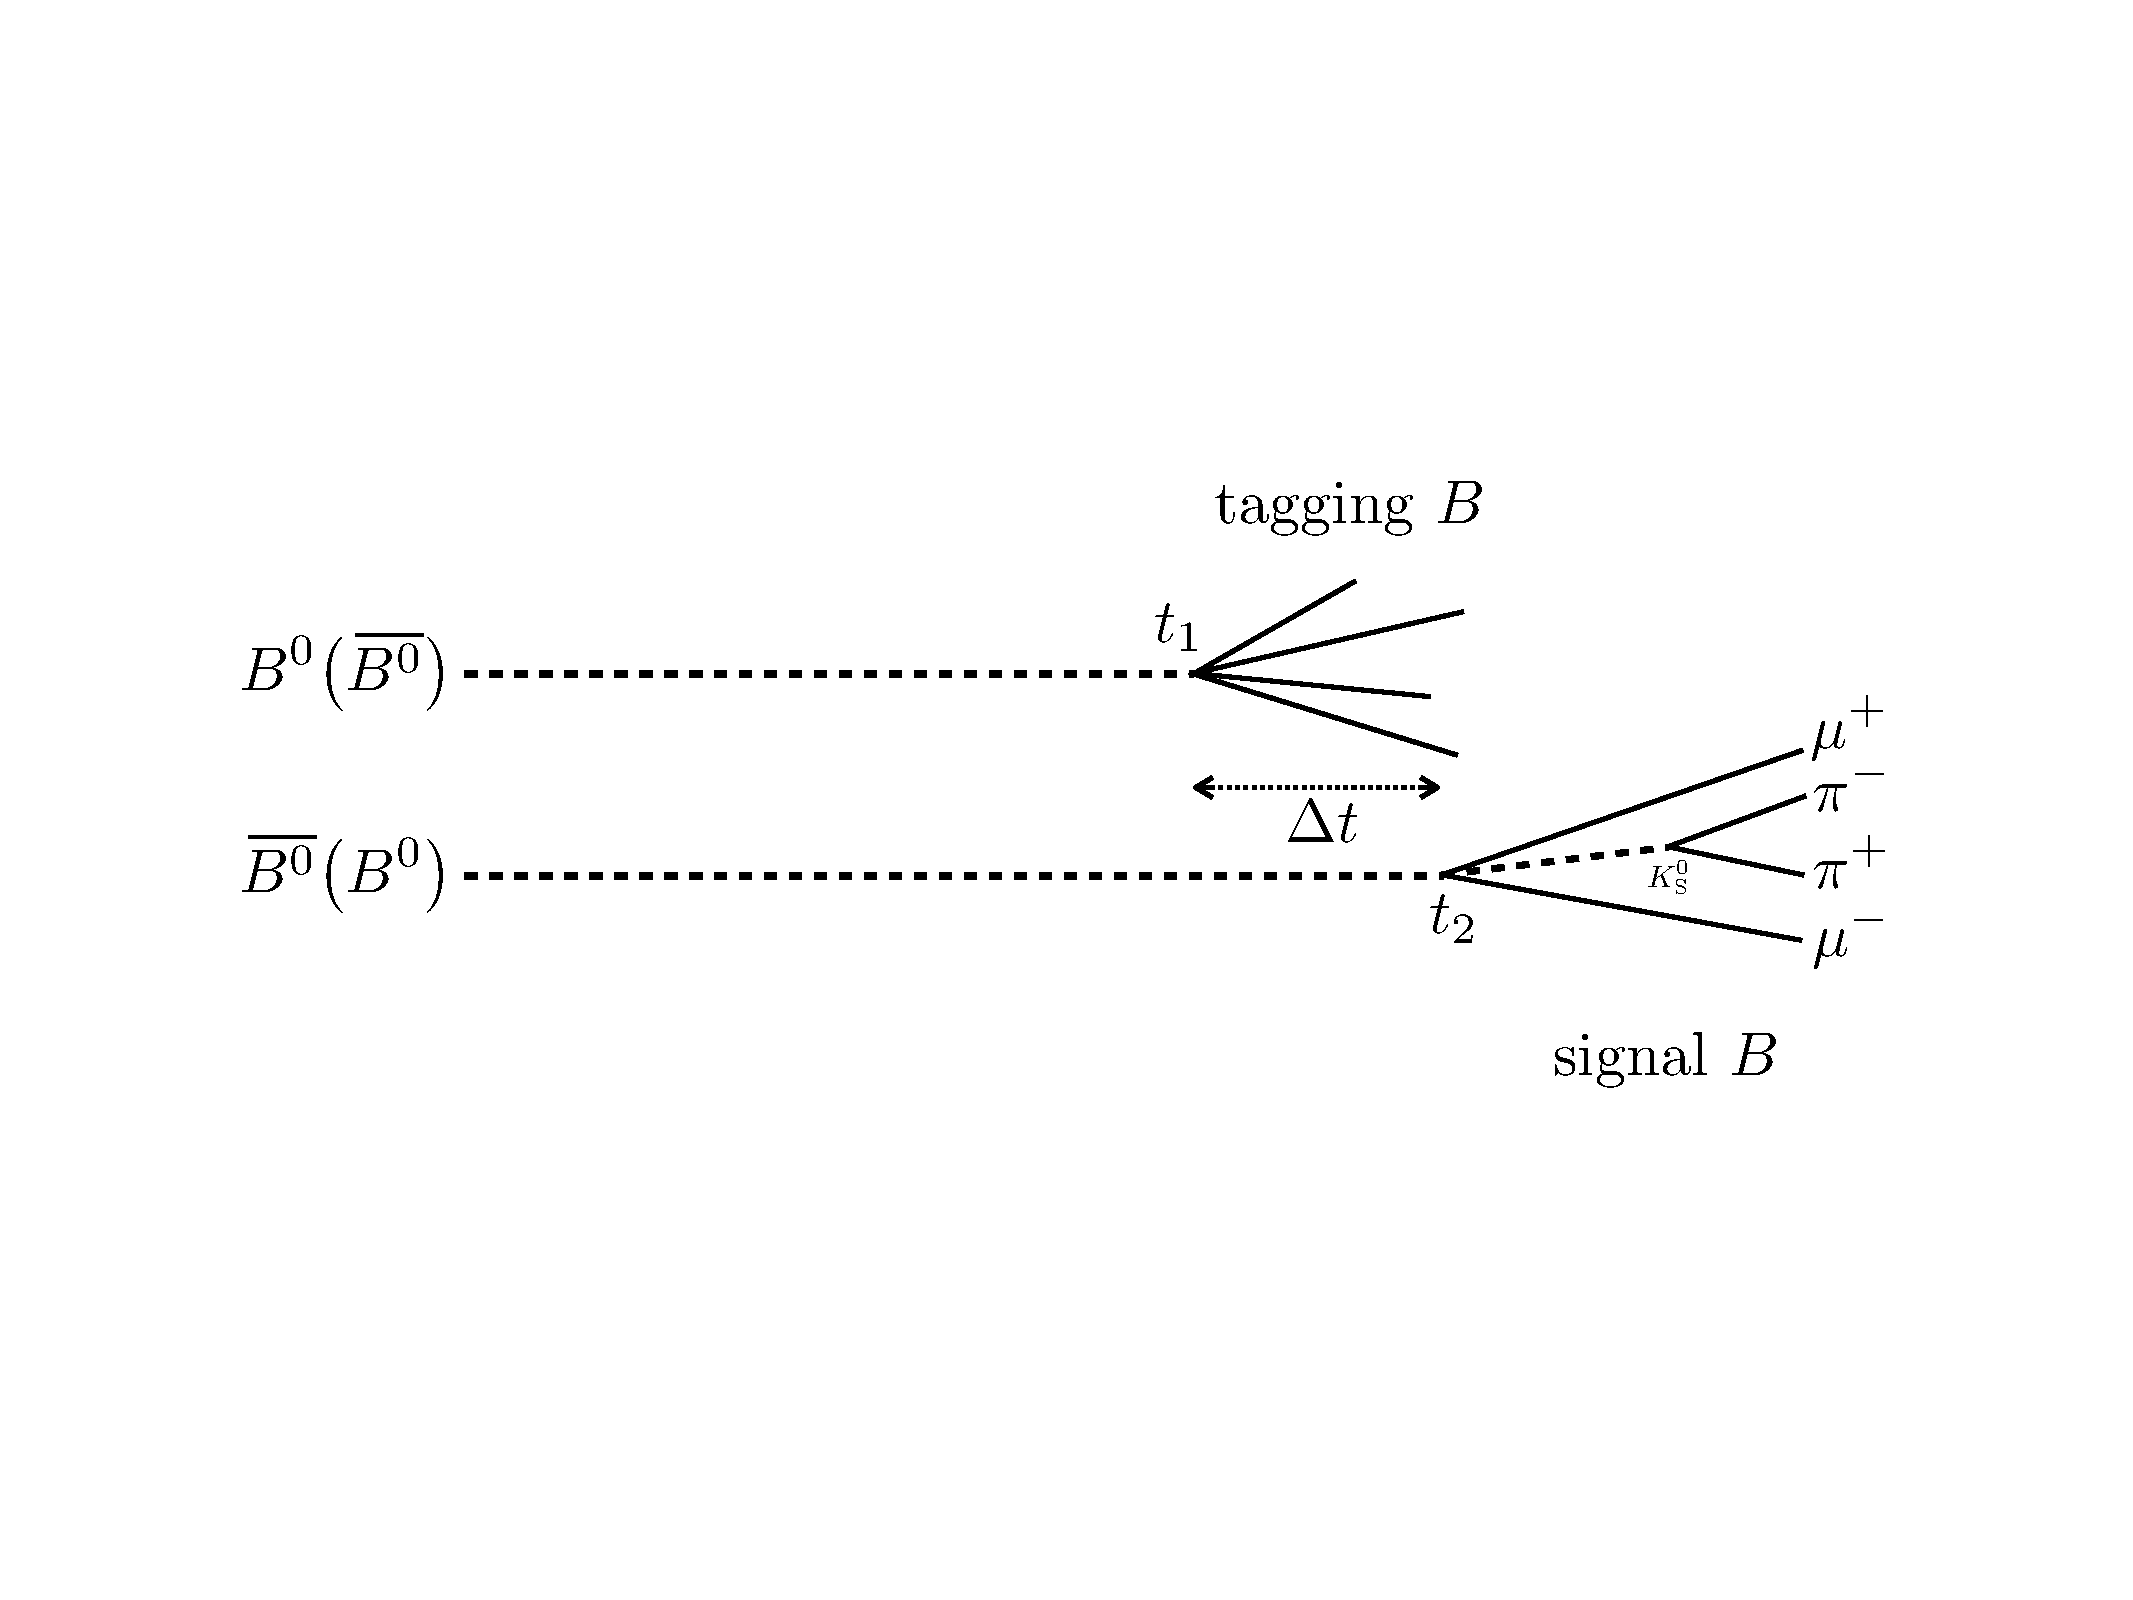
\includegraphics[width=\textwidth]{private/content/flavour-tagging/figs/bfactory_tagging}
\caption{Illustration of the measurement of \sintwobeta as conducted by the \BFactories.
}
\label{fig:flavour_tagging:lhcb:b_factory_basic_principles}
\end{figure}

\Cref{fig:flavour_tagging:lhcb:b_factory_basic_principles} illustrates the basic
principles of a \CP violation measurement at the \BFactories. The produced
$\Bd\Bdbar$ pair's wave function is in a $P$-wave entangled state, until one of
the mesons decays. From this point in space time ($t_1$) the second $\B$ meson
propagates further through the detector, mixes to its antimatter state, and
finally decays at $t_2$. The \CP asymmetry $\CPAsymmetry$ will therefore be a
function of the decay time difference $\Delta t$. This has two implications:
First, the decay time difference will always be computed relative to the
\enquote{tagging} \Bmeson decay and thus might be negative if the signal $\B$
meson decays first. Secondly, if the tagging \Bmeson decays into a
flavour-specific final state, this specifies the signal \Bmeson's flavour at
$\Delta t=0$.

As a result of the production mechanism, the fully reconstructed signal decay
leaves all remaining tracks to originate from the tagging $\B$. This allows to
classify the decay of the tagging meson according to the signature of the final
state particles. Specialised taggers then identify decays based on their
specific signature. In a second stage, all results provided by the single
taggers are combined into a final tagging decision. 

The lepton taggers deduce a tag from the charge of electrons and muons from
$\bquark \to \cquark \lepm \neutrinobar$ transitions in semileptonic $\B$
decays. Likewise, second order transitions from $\bquark \to \Wm \cquark ( \to
\squark \lepp \neutrino )$ can be used, but have to be handled differently as
their charge is opposite compared to primary leptons. Charged kaon candidates
from the $\bquark \to \cquark \to \squark$ decay chain reflect the charge of the
tagging meson. Here as well, kaons from second order transitions carry the
opposite charge. Charged pions from charm decays work as tagging particles
either directly or in events with both a pion and a charged kaon, the
correlation of the particles can be utilised to improve the tag decision.
Selecting high momentum particles, \eg fast pions from $\Bdbar \to \Dstarp
\pim$, is on its own another source of tagging information and might
additionally be correlated with slow particles to enhance the tagging result.
Finally the flavour of $\Lambda$ baryons from decays of the tagging $\B$ meson
can be exploited.

The \Babar experiment uses \acp{ANN} for each single tagger to provide several
intermediate tagging decisions that are subsequently combined using another \ANN
to gain a joined tagging decision. The effective tagging efficiency of the final
\Babar tagging algorithm is estimated on data to be $\efftageff = \SI{33.1 +-
0.3}{\percent}$. In \Belle analyses the flavour tagging approach is similar.
Instead of \acp{ANN} multi-dimensional look-up tables are used. At first,
information from charged tracks are looked-up to sort them into the signature
categories. Next, the received results are used on an event-level to provide the
final tagging decision. Using this approach an effective tagging efficiency of
$\efftageff = \SI{30.1 +- 0.4}{\percent}$ is achieved.

% ------------------------------------------------------------------------------
\subsection{\Acl{OS} algorithms}
\label{sec:flavour_tagging:os}

The \OS algorithms all infer the tagging decision from the quark flavour of the
\bhadron produced in association with the signal \Bmeson. If for example a $\Bu$
decays into a $\Kp X$ final state trough $\bquarkbar \to \cquarkbar \to
\squarkbar$ transition, it can unambiguously stated by looking at the kaon
charge that the \bhadron produced along with the $\Bu$ contained a $\bquark$
quark. The tag identification for events with this signature fall into the scope
of the \OSK tagger.

In total four distinct \OS taggers, each developed for a special \OS decay
signature, provide tagging information. Besides the \OSK tagger, the \OSe and
the \OSm taggers select leptons coming from the primary $\bquark \to X \lepm$
decay to use their charge as an information carrier of the $\B$ flavour.
Finally, the \OSvtx tagger performs an inclusive reconstruction of the \OS \SV
to then compute a weighted sum of all particle track charges that originate from
the \SV. In the following the selection criteria and algorithms of the \OS
taggers are briefly described.

\missing{Intrinsic mistag due to neutral B meson oscillation}
 
%...............................................................................
\subsubsection{The \acl{OSK} tagger}
\label{sec:flavour_tagging:os:kaon}

The kaon tagger exploits the charge of kaons stemming from $\bquark \to
\cquark \to \squark$ decays of the opposite side \bhadron. As the charge of the
kaon is the same of the ancestor's charge, the kaon always carries the opposite
charge as the signal \Bmeson.

To reduce background contributions of prompt kaons and kaons from primary
$\bquarkbar \to \Wm (\to \cquark \squarkbar) \cquarkbar$ transitions, in which
case the kaon carries the \enquote{wrong} charge, several selection criteria are
applied. Cuts on the \pT, the \IP, the \IP/$\sigma_\text{\IP}$, and the track
fit \chisqndf are performed. \PID requirements on the \DLLKpi, the \DLLppi, and
\DLLmupi suppress mis-identified particles. Clone tracks are removed and kaon
candidates with originate from other \acp{PV} are rejected using a cut on the
\IP/$\sigma_\text{\IP}$ with respect to any \PV.
\cref{tab:flavour_tagging:os:kaon:cuts} lists all applied cuts. If more than one
tagging candidate is found, the decision obtained from the candidate with the
highest \pT is chosen. To further increase the effective tagging efficiency only
tag decisions are considered if the estimated mistag probability is smaller than
$\mathcal{P}=0.46$.

\begin{table}
  \centering
  \caption{Selection cuts for the \OSK tagger \cite{Grabalosa:2012qra}.}
  \label{tab:flavour_tagging:os:kaon:cuts}
  \begin{tabular}{ll}
    \toprule
    Property & Value \\
    \midrule
    \pT                                       & $>\SI{0.5}{\GeVc}$                  \\
    \IP                                       & $<\SI{1.25}{\milli\metre}$          \\
    \IP$/\sigma_\text{\IP}$                   & $>\num{3.35}$                       \\
    track fit \chisqndf                       & $<\num{2.75}$                       \\
    \DLLKpi                                   & $>\num{6}$                          \\
    $(\DLLKpi - \DLLppi)$                     & $>\num{-4}$                         \\
    \IP$/\sigma_\text{\IP}$ \wrt any \PV      & $>\num{4.5}$                        \\
    reject clone tracks & \\
    \bottomrule
  \end{tabular}
\end{table}

%...............................................................................
\subsubsection{The \acl{OSe} and the \acl{OSm} taggers}
\label{sec:flavour_tagging:os:lepton}

Leptons from $\bquark \to \cquark\Wboson$ transitions are selected in order to
deduce the opposite \bhadron charge. Thus positive lepton charge indicates a
$\bquark$ quark content of the signal \Bmeson and vice versa.

Cuts on the \PID and the lepton \pT are applied to reduce the mis-identification
rate and to suppress leptons from secondary decays of charm mesons. The muon
candidate purity is further enhanced by reducing fake muons, clone tracks, and
requiring a sufficient track fit quality. Electron candidate tracks must lie
inside the \HCAL acceptance and leave a substantial energy deposition in the
\ECAL compared to their momentum. To reduce backgrounds from photon conversions
close to the \protonproton interaction region, a upper limit on the maximal
ionisation charge $Q_\text{\VELO}$ deposited in the \VELO is set. If more than
one lepton candidate passes the requirements, the one with the highest \pT is
chosen. The selection cuts for the lepton taggers are listed in
\cref{tab:flavour_tagging:os:lepton:cuts}.
%
\begin{table}
  \centering
  \caption{Selection cuts for the \OSe and \OSm taggers
  \cite{Grabalosa:2012qra}, where $E$ is the particle energy measured in the
  \ac{ECAL} and $p$ the measured particle momentum. $Q_\text{\VELO}$ describes
  the ionisation charge deposit in the \VELO.}
  \label{tab:flavour_tagging:os:lepton:cuts}
  \begin{tabular}{ll}
    \toprule
    % general
    Property                                  & Value                               \\
    \midrule
    lepton \pT                                & $>\SI{1.2}{\GeVc}$                  \\
    muon \DLLmupi                             & $>\num{1}$                          \\
    muon track fit \chisqndf                  & $<\num{3.2}$                        \\
    \multicolumn{2}{l}{reject muon clone tracks and fake muons}                     \\
    electron \DLLepi                          & $>\num{4}$                          \\
    electron $E/p$                            & $>\num{0.8}$                        \\
    max. electron $Q_\text{\VELO}$            & $<\num{1.6}$                        \\
    \multicolumn{2}{l}{electron candidate track in \HCAL acceptance}                \\
    \bottomrule
  \end{tabular}
\end{table}

%...............................................................................
\subsubsection{The \acl{OSvtx} tagger}
\label{sec:flavour_tagging:os:vertex}

Besides the single particle taggers for kaons, muons, and electrons, the
\ac{OSvtx} tagger follows an alternative approach by trying to inclusively
reconstruct the decay vertex of the opposite \bhadron. Starting with a two-track
seed, matching tracks are appended and a weighted sum of the vertex charge is
calculated. The procedure is optimized using cuts on the considered tracks, the
seed properties, and the features of the reconstructed vertex.

The initial vertex seed is found by sampling track pairs from all particle
candidates surviving the following criteria: At least one of the tracks must be
a long track with a track fit quality of $\chisqndf<\num{2.5}$. To exclude poor
track reconstruction only tracks with an \IP (\wrt the \PV) uncertainty of
$\sigma_\text{\IP}<\num{1}$ are taken into account. Tracks from prompt particles
are rejected if the \IP significance $\text{\IP}/\sigma_\text{\PV}$ \wrt the \PV
is below $\num{2.5}$ or above $\num{100}$. Additionally the track has to have a
$\pT>\SI{0.15}{\GeVc}$ and an \IP$<\SI{3}{\milli\metre}$ \wrt to the \PV. The
two seed tracks must be separated by an angle of $\phi>\SI{1}{\mrad}$ and one of
the tracks has to have a $\pT>\SI{0.3}{\GeVc}$.

For tracks pairs passing all selection criteria a vertex fit is performed. If
the fit succeeds and a fit quality of at least $\chisqndf<10$ is met, the fitted
vertex is considered as a seed. The seed is required to lie inside the detector
acceptance and in the forward direction of the \PV ($z>0$). 

The invariant mass of the seed is calculated and has to be greater than
$\SI{0.2}{\GeVcc}$ and not be compatible with the known $\KS$ or $\Lambdaz$
masses. % 0.490 < m_KS < 0.505 and 1.11 < m_Lambda < 1.12
A likelihood is computed for all seeds considering the vertex fit $\chisqndf$,
the minimum \pT, the maximum \PV \IP, the minimum \PV \IP$/\sigma_\text{\IP}$,
the angle between the seed tracks, the $z$-distance to \PV, and the angle
between the seed direction \wrt to the \PV. The seed with the maximum likelihood
is selected. The seed algorithm successfully finds a seed in nearly
$\SI{50}{\percent}$ of all events and has a rate of $\SI{60}{\percent}$ to find
a seed that is formed by \bhadron decay products.

Subsequently more tracks are added to the seed. Additional tracks are required
to be compatible with the reconstructed seed vertex
(\IP$<\SI{0.9}{\milli\metre}$), have a \DOCA to any track in the seed smaller
than $\SI{0.2}{\milli\metre}$, the track fit quality is at least
$\chisqndf<\num{3}$, and are ruled out to be a clone track. Additionally the \IP
with respect to the \PV has to be larger than $\SI{0.1}{\milli\metre}$ and
$\text{\IP}/\sigma_\text{\IP}>\num{3.5}$.

After all tracks are added to the vertex another set of selection requirements
has to be fulfilled to optimize the effective tagging efficiency. The sum of all
track momenta has to be $\sum_i p_i > \SI{10}{\GeVc}$ and $\sum_i \pT(i) >
\SI{10}{\GeVc}$, the invariant vertex mass must be greater than $m_\text{vtx} >
\SI{0.5}{\GeVcc}$, the sum of the track
$\sum_i\text{\IP}_i/\sigma_{\text{\IP}_i}$ has to be larger $\num{10}$ and the
sum of the track \DOCA has to be $\sum_i\text{\acs{DOCA}}_i <
\SI{0.5}{\milli\metre}$.

The tag decision is then deduced from the inclusively reconstructed vertex by
calculating the weighted charge for all tracks $i$ forming the vertex
%
\begin{equation}\label{eq:flavour_tagging:os:vertex:charge}
  Q_\text{vtx} = \frac{\sum_i \pT^k(i)Q_i}{\sum_i\pT^k(i)}\eqcm
\end{equation}
where the track \acp{pT} are used as weights and the $k$ parameter is optimised
using simulated data to be $k=\num{0.4}$. In a final step, only charges of
$\vert Q_\text{vtx} \vert > 0.25$ are considered and the mistag probability has
to be smaller than $\mathcal{P}=0.46$.

% ------------------------------------------------------------------------------
\subsection{\Acl{SS} algorithms}
\label{sec:flavour_tagging:ss}

The \acl{SS} taggers exploit charge information from pions or kaons produced in
the hadronisation process of the signal \Bmeson. As illustrated in
\cref{fig:flavour_tagging:lhcb:schematics} the $\qqbar$ quark pair produced
alongside the signal meson, splits up to form the $\B$ meson and in the case of
a $\Bd$ ($\Bs$) an accompanying pion (kaon). Pions might also be produced in the
decay of excited $\B$ meson states.

%...............................................................................
\subsubsection{The \acl{SSpi} tagger}
\label{sec:flavour_tagging:ss:pion}

The pions from either the \Bmeson hadronisation or the decay of excited states
carry the same charge as the signal \Bmeson and are therefore suitable to
extract tagging information. The selection criteria pion candidates are required
to fulfil are listed in \cref{tab:flavour_tagging:ss:pion:cuts}. If more than
one pion candidate passes the requirements, the one with the highest \pT is
chosen. The tag decision has to have a mistag probability of $\mathcal{P}<0.46$,
otherwise it will be refused.
%
\begin{table}
  \centering
  \caption{Selection cuts for the \SSpi tagger \cite{Grabalosa:2012qra}, where
  $\Delta Q$ describes the mass difference of the $\Bd\pion$ mass and the $\Bd$
  mass.}
  \label{tab:flavour_tagging:ss:pion:cuts}
  \begin{tabular}{ll}
    \toprule
    Property                                  & Value                               \\
    \midrule
    \multicolumn{2}{l}{only long track pion candidates}                             \\
    \DLLKpi                                   & $<\num{4.5}$                        \\
    \DLLppi                                   & $<\num{15}$                         \\
    \pT                                       & $>\SI{0.5}{\GeVc}$                  \\
    $p$                                       & $>\SI{2.5}{\GeVc}$                  \\
    \PV $\text{\IP}/\sigma_\text{\IP}$        & $<\num{4}$                          \\
    $\Delta Q$                                & $<\SI{1.5}{\GeVcc}$                 \\
    \bottomrule
  \end{tabular}
\end{table}

%...............................................................................
\subsubsection{The \acl{SSK} tagger}
\label{sec:flavour_tagging:ss:kaon}

The charge of kaons produced together with a signal $\Bs$ meson can be exploited
in order to get a tag decision. The selection requirements for kaon candidates
are similar to those for the \SSpi tagger. Besides \PID variables, momenta, the
quality of the \IP fit and the track fit, differences between the $\Bs\kaon$
mass and the $\Bs$ mass, the difference in the $\phi$ angle between the signal
\Bmeson and the kaon, and the pseudo-rapidity between the signal \Bmeson and the
kaon are taken into account. If more than one candidate passes the criteria, the
one with the highest \pT is used. As this thesis presents a measurement in the
decay of $\Bd$ and $\Bdbar$ mesons, where the kaon tagger is not used.
% , no further details will be given and an emphasis is placed on the \SSpi tagger.
% %
% \begin{table}
%   \centering
%   \caption{Selection cuts for the \SSK tagger \cite{Grabalosa:2012qra}, where
%   $\Delta Q$ describes the mass difference of the $\Bs\kaon$ mass and the $\Bs$
%   mass, $\vert \Delta\phi \vert$ the difference in the $\phi$ angle between the
%   signal \Bmeson and the kaon, $\vert \Delta\eta \vert$ the pseudo-rapidity
%   between the signal \Bmeson and the kaon, and $\vert \Delta R \vert =
%   \sqrt{\Delta\eta^2 + \Delta\phi^2}$.}
%   \label{tab:flavour_tagging:ss:kaon:cuts}
%   \begin{tabular}{ll}
%     \toprule
%     Property                                  & Value                               \\
%     \midrule
%     \DLLKpi                                   & $>\num{4.5}$                        \\
%     (\DLLKpi - \DLLppi)                       & $>\num{-8.5}$                       \\
%     \pT                                       & $>\SI{0.75}{\GeVc}$                 \\
%     $p$                                       & $>\SI{5.25}{\GeVc}$                 \\
%     \PV $\text{\IP}/\sigma_\text{\IP}$        & $<\num{4.125}$                      \\
%     track $\chisqndf$                         & $<\num{3.75}$                       \\
%     $\Delta Q$                                & $<\SI{1.5}{\GeVcc}$                 \\
%     $\vert \Delta\phi \vert$                  & $<\num{0.7}$                        \\
%     $\vert \Delta\eta \vert$                  & $<\num{0.525}$                      \\
%     $\vert \Delta R \vert$                    & $<\num{1.2}$                        \\
%     \bottomrule
%   \end{tabular}
% \end{table}

% %%%%%%%%%%%%%%%%%%%%%%%%%%%%%%%%%%%%%%%%%%%%%%%%%%%%%%%%%%%%%%%%%%%%%%%%%%%%%%
\section{Calibration of the flavour tagging output}
\label{sec:flavour_tagging:calibration}

The tagging decisions each tagger estimates are based on selection criteria
developed using simulations and flavour-specific decays. While the tag decision
$d$ depends on a measured particle or vertex charge, the mistag estimate
$\mistagestimate$ is computed using \acp{ANN} trained on \sweighted $\BuToJpsiK$
data incorporating kinematic and geometric event properties.

In order to adjust for differences between the training and physics data, the
\ANN output is calibrated using flavour-specific decays. For the \OS taggers and
the \SSpi tagger, $\BuToJpsiK$ decays are used to develop a calibration function
$\omofeta$ (while the data sample that was used to train the \ANN before is
omitted). Decays of charged \Bmesons are not subject to quark mixing, thus, the
true mistag probability $\omega$ can be determined directly by counting and
comparing the final state charges. In case of neutral $\B$ decays into
flavour-specific final states a full time-dependent mixing analysis is
necessary.

In \cref{sec:flavour_tagging:calibration:method} general concepts and the choice
of the calibration function are presented, then the methodologies of a
calibration using decays of either charged or neutral \Bmesons is explained. Two
different approaches how to incorporate the per-event tagging information are
described and an outlook into the technique of combining different tagger's
output into a single tag decision is given. Then the calibration of the \OS and
the \SSpi taggers using $\BuToJpsiK$ and $\BdToJpsiKstar$ decays is shown in
\cref{sec:flavour_tagging:calibration:os,sec:flavour_tagging:calibration:ss}.

% ------------------------------------------------------------------------------
\subsection{Methodology}
\label{sec:flavour_tagging:calibration:method}

The calibration of the flavour tagging output usually follows an iterative
procedure. All single taggers and the combination of all \OS tagging decisions
(see \cref{sec:flavour_tagging:combination}) is calibrated using the high yield
decay channel $\BuToJpsiK$. The correction determined in this step is then
applied to the tagging algorithms during the common data processing stage
(\enquote{Stripping}). Afterwards, the calibration is checked on several control
channels, \ie $\BuToJpsiK$, $\BuToDpi$, $\BdToJpsiKstar$, $\BdToDpi$,
$\BdToDstarmunu$ and $\BsToDspi$ and possible small corrections can be applied
for individual analyses. Assuming no correlations amongst the single taggers, it
can be assumed, that the calibration is still valid for the combined tagging
estimates. This assumption is checked as well.

The calibration function $\omofeta$ is chosen linear with two parameters
$\pzero$ and $\pone$,
%
\begin{equation}\label{eq:flavour_tagging:calibration:method:calibration}
  \omofeta = \pzero + \pone (\mistagestimate - \avgmistagestimate)\eqcm
\end{equation}
%
with $\avgmistagestimate$ being the average mistag estimate used to decorrelate
$\pzero$ and $\pone$. Hence, a perfect calibrated tagging output would result in
$\pzero = \avgmistagestimate$ and $\pone = 1$. The performance of the tagging
algorithms may depend on the flavour of the initial \Bmeson. Different
interaction of particles, \eg kaons used by the \OSK tagger, induce deviating
reconstruction efficiencies, resulting in different tagging efficiencies
$\tageff$ and mistag probabilities $\mistag$ for initial $\Bd$ and $\Bdbar$
states. To correct for asymmetries of the tagging calibration $\deltamistag =
\mistag^{\Bd} - \mistag^{\Bdbar}$ and two independent calibration functions are
defined
%
\begin{equation}\label{eq:flavour_tagging:calibration:method:asymmetric_calibration:omega}
  \begin{split}
    \omofetaBd    &= \pzeroBd    + \poneBd    (\mistagestimate - \avgmistagestimate)\eqcm \\
    \omofetaBdbar &= \pzeroBdbar + \poneBdbar (\mistagestimate - \avgmistagestimate)\eqcm
  \end{split}
\end{equation}
%
where the calibration parameters $\p{i}{}$ (with $i=0,1$) can be parametrised as
%
\begin{equation}\label{eq:flavour_tagging:calibration:method:asymmetric_calibration:ps}
  \p{i}{\Bd} = \p{i}{} + \frac{\deltap{i}{}}{2} \eqspace\text{and}\eqspace \p{i}{\Bdbar} = \p{i}{} - \frac{\deltap{i}{}}{2}\eqpd
\end{equation}

%...............................................................................
\subsubsection[Flavour tagging calibration using decays of charged \Bmesons]{Flavour tagging calibration using decays of charged \Bbfsf mesons}
\label{sec:flavour_tagging:calibration:method:charged}

Using decays of charged \Bmesons into flavour-specific final states like
$\BuToJpsiK$ and $\BuToDpi$ is the straightforward way to calibrate the flavour
tagging. The decisions given by the tagging algorithms can be easily compared to
the final state charges without ambiguities due to oscillations in the \Bmeson
system.

Using a fit to the $\Bu$ mass distribution the background contributions can be
subtracted using the \sPlot technique \cite{Pivk:2004ty}. The mistag estimate
distribution can then be split into $n$ bins to compare the average estimated
mistag of each bin $\mistagestimate_i$ to the counted mistag ratio $\mistag_i$.
\Cref{fig:flavour_tagging:calibration:method:charged:calibration_plot} shows an
exemplary calibration plot using a dataset of $\BuToJpsiK$ decays corresponding
to an integrated luminosity of $\SI{0.37}{\per\femtobarn}$ \cite{Aaij:2012mu}.
The data is categorised into $\num{21}$ bins of $\mistagestimate$ and a linear
function is fit to the data to estimate the calibration parameters $\pzero$ and
$\pone$.
%
\begin{figure}
\centering
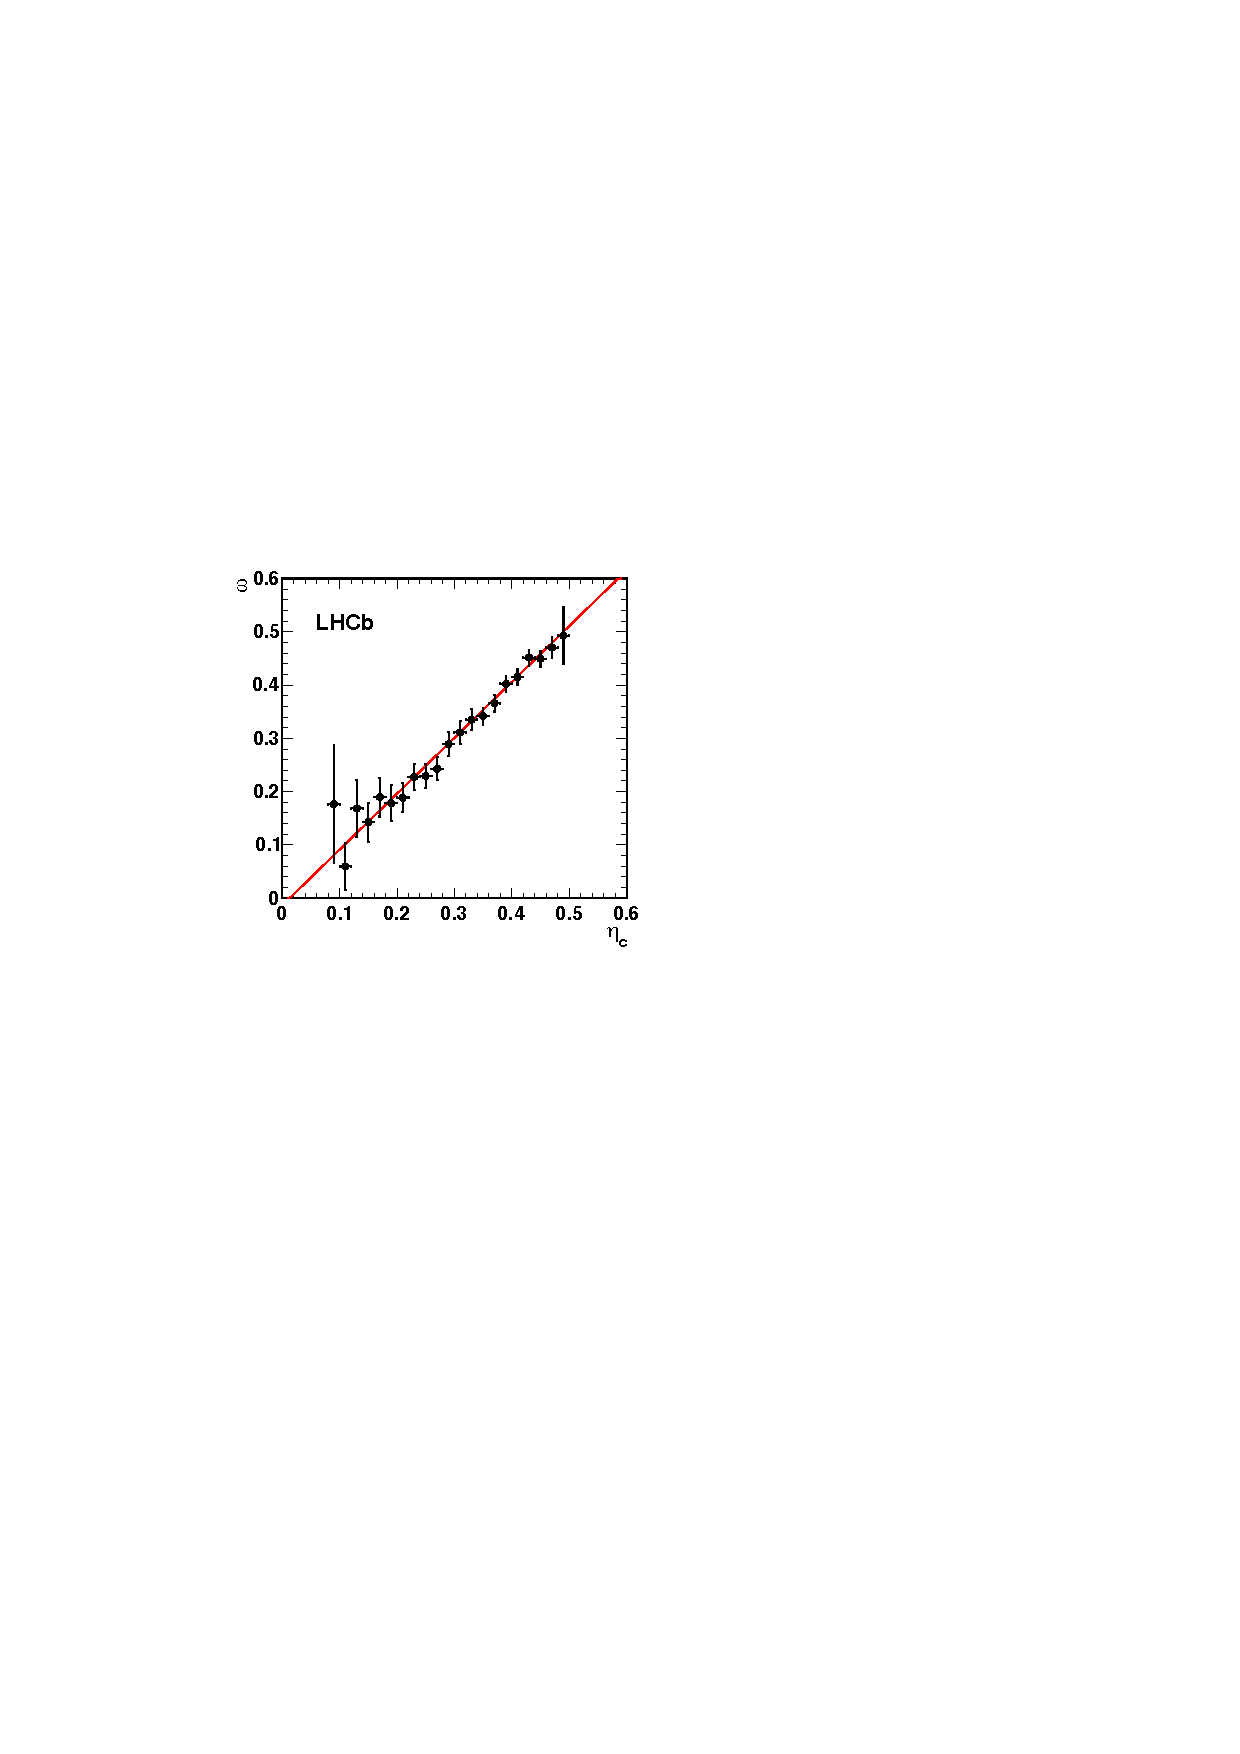
\includegraphics[width=0.5\textwidth]{private/content/flavour-tagging/figs/lhcb_ft_calibration_bu2jpsik_037fb}
\caption{Measured mistag fraction $\mistag$ plotted against the mistag estimate
$\mistagestimate$ provided by the tagging algorithms. Described in black are
data of $\BuToJpsiK$ decays corresponding to an integrated luminosity of
$\SI{0.37}{\per\femtobarn}$. The red line illustrates the linear calibration
function fitted to the data. \cite{Aaij:2012mu}}
\label{fig:flavour_tagging:calibration:method:charged:calibration_plot}
\end{figure}

As an alternative, the calibration function can be implemented into the unbinned
maximum likelihood fit to the dimensions: mass, tagging decision, and mistag
probability estimate. Using a conditional \PDF
$\Prob{}{\Sig}(\tagdecision,\tagdecision^\prime,\mistagestimate)$, where
$\tagdecision^\prime$ describes the true $\Bu$ tag derived from the final-state
particle charge.
%
\begin{equation}\label{eq:flavour_tagging:calibration:method:charged:tagdefinition}
  \Prob{}{\Sig}(\tagdecision,\tagdecision^\prime,\mistagestimate) = 
  \begin{cases}
        \tageff (1-\omofeta) \Prob{}{\Sig}(\mistagestimate)    & \text{if $\tagdecision =    \tagdecision^\prime$} \\
        \tageff    \omofeta  \Prob{}{\Sig}(\mistagestimate)    & \text{if $\tagdecision \neq \tagdecision^\prime$} \\
    1 - \tageff                                                & \text{if $\tagdecision = 0$} \\
  \end{cases}
\end{equation}
%

%...............................................................................
\subsubsection{Flavour tagging calibration using decays of neutral \Bmesons}
\label{sec:flavour_tagging:calibration:method:neutral}

In the decay of neutral \Bmesons the oscillation of the propagating $\B$ state
prevents the determination of the initial flavour just by measuring the final
state charge. Instead a full decay time dependent mixing analysis has to be
performed. As described \eg in \cite{Aaij:2012nt} the signal mixing asymmetry is
given by
%
\begin{equation}
  \MixingAsymmetry = (1 - 2\mistag)\cos(\DMd t)\eqpd
\end{equation}
%
This can be either utilised in a simultaneous fit in different bins of
$\mistagestimate$ to extract per bin $\mistag_i$, then following the same
procedure as described for charged initial states or by implementing the
calibration function $\omofeta$ directly into the \PDF.

%...............................................................................
\subsubsection{Evaluation of systematic uncertainties}
\label{sec:flavour_tagging:calibration:method:systematics}

In the determination of systematic uncertainties two different causes of errors
are considered: \enquote{type I} uncertainties are related to systematic
uncertainties from the methodology of the calibration itself, while
\enquote{type II} uncertainties account for systematic uncertainties resulting
from using the calibration parameters determined in a control channel in the
signal channel.

% ------------------------------------------------------------------------------
\subsection[
  head={\ac{OS} tagger calibration using \BuToJpsiK decays},
  tocentry={\ac{OS} tagger calibration using \BuToJpsiKHyperref decays}
]{\ac{OS} tagger calibration using \BuToJpsiKbfsf decays}
\label{sec:flavour_tagging:calibration:os}

Deviating from the standard procedure to calibrate the \OS taggers and their
combination using a set of physics channels, only $\BuToJpsiK$ is used. A
previous study \cite{Aaij:1497268} made apparent that the uncertainties arising
from the flavour tagging calibration provide the largest contribution to the
overall systematic uncertainties on the measured quantities $\SJpsiKS$ and
$\CJpsiKS$. Therefore, going without semileptonic and fully hadronic decay modes
with different kinematic properties and only use $\BuToJpsiK$ decays with a
nearly similar final state, can reduce the uncertainties. An additional
cross-check of the calibration is performed on $\BdToJpsiKstar$ decays to
confirm the portability of the calibration on a $\Bu$ to a $\Bd$ initial state.
\missing{\OS calibration: $\BuToJpsiK$ data sample and signal selection}

The calibration then follows the already outlined approach: extracting \sweights
by a fit to the \Bu mass distribution, then comparing the true fraction of wrong
tagged candidates to the average mistag estimate in $\num{60}$ $\mistagestimate$
bins. The mass model used in the fit is a sum of three Gaussian \acp{PDF} with a
shared mean to describe the signal shape and an exponential \PDF for the
background contributions. The fit to the $(\mistagestimate_i,\mistag_i)$ pairs
using \cref{eq:flavour_tagging:calibration:method:calibration} yields
%
\begin{equation}\label{eq:flavour_tagging:calibration:os:parameters}
  \begin{split}
    \p{0}{\text{\acs{OS}}} &= 0.3815 \pm 0.0011 \text{\,(\stat)} 
                               \pm 0.0015 \text{\,(\syst type I)}  
                               \pm 0.0005 \text{\,(\syst type II)} \eqcm\\ % total syst 0.0016 
    \p{1}{\text{\acs{OS}}} &= 0.978\phantom{0} \pm 0.012\phantom{0} \text{\,(\stat)} 
                                         \pm 0.006\phantom{0}  \text{\,(\syst type I)} 
                                         \pm 0.007\phantom{0}  \text{\,(\syst type II)} \eqcm\\ % total syst 0.009
    \langle\mistagestimate^{\text{\acs{OS}}}\rangle &= 0.3786 \eqcm \\
    \rho_{\pzero,\pone} &= 0.14 \eqcm
  \end{split}
\end{equation}
%
where $\rho_{\pzero,\pone}$ is the correlation between $\p{0}{\text{\acs{OS}}}$ and
$\p{0}{\text{\acs{OS}}}$. \Cref{fig:flavour_tagging:calibration:os:mass_and_calibration}
shows the mass distribution and the \PDF projection as well as the calibration
plot.
%
\begin{figure}
  \centering
  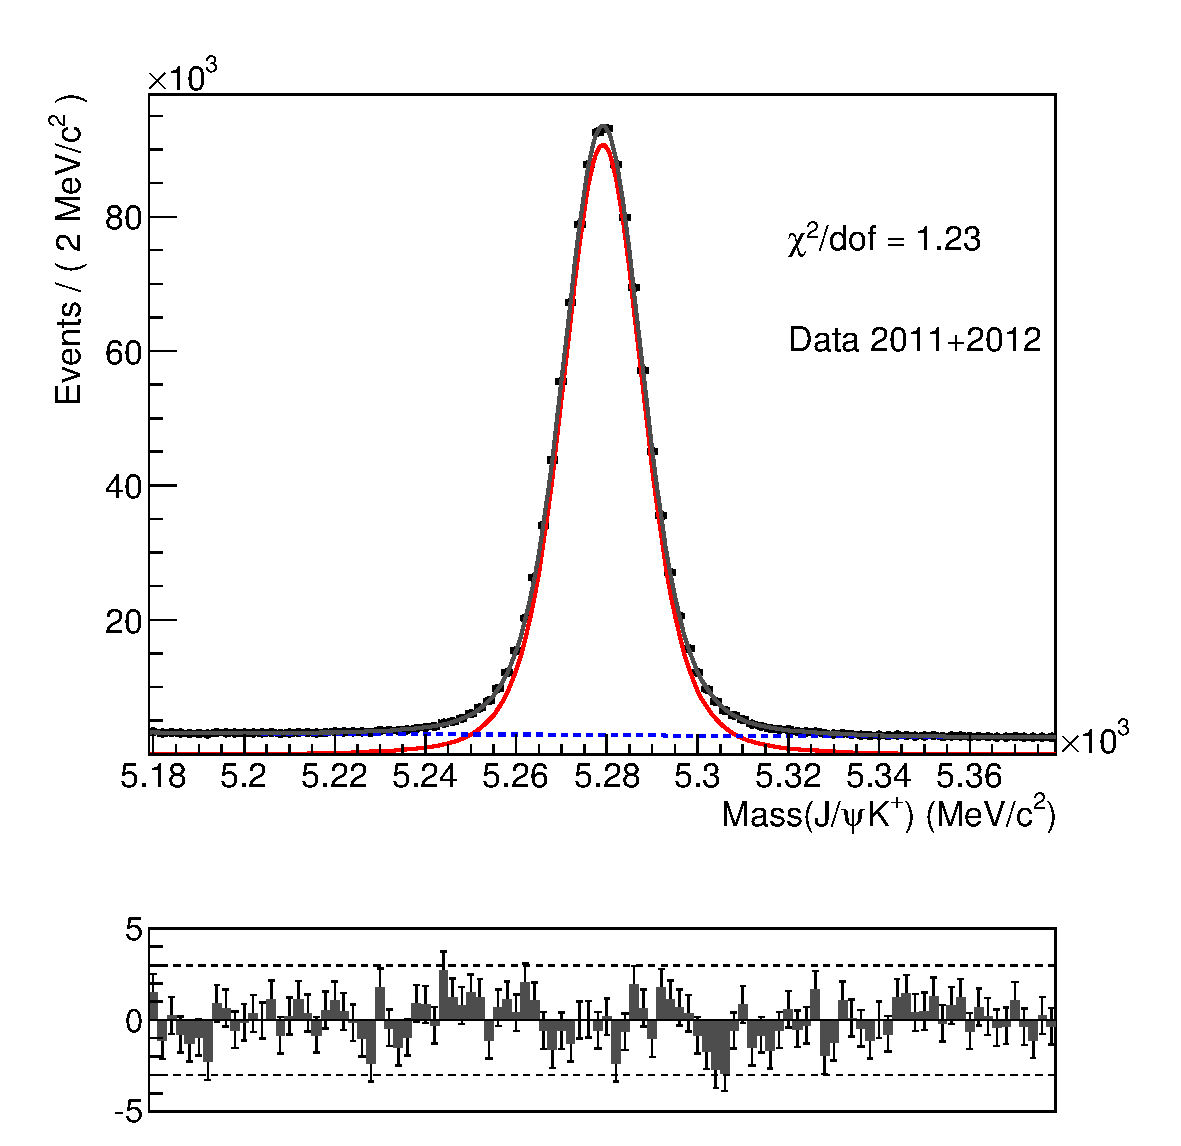
\includegraphics[width=0.48\textwidth]{private/content/flavour-tagging/figs/lhcb_ft_calibration_bu2jpsik_mass}
  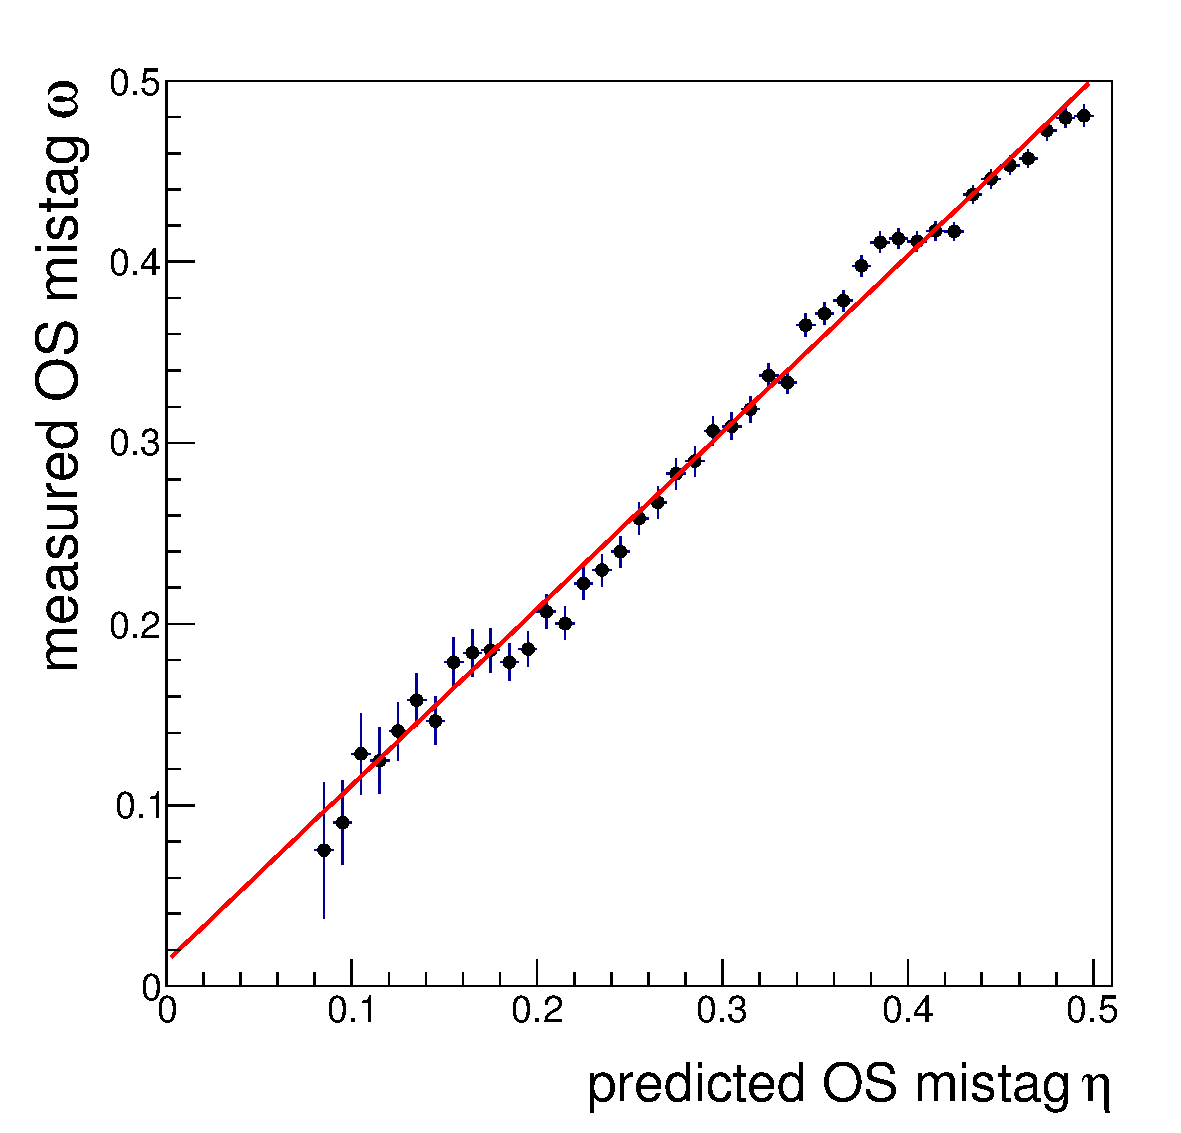
\includegraphics[width=0.48\textwidth]{private/content/flavour-tagging/figs/lhcb_ft_calibration_bu2jpsik_calibration}
  \caption{(Left) Distribution of $\BuToJpsiK$ mass and projection of the fit \PDF.
  The black solid line shows the total mass \PDF, the red solid line the signal
  and the blue dashed line the background component. (Right) Distribution of
  $(\mistagestimate_i,\mistag_i)$ pairs in the decay $\BuToJpsiK$ together with
  the linear calibration function in red. \cite{FT:RunI}}
  \label{fig:flavour_tagging:calibration:os:mass_and_calibration}
\end{figure}
%
The asymmetries in the mistag probabilities are determined by repeating the
measurement when splitting the data sample into the initial $\Bd$ flavours and
comparing the values for $\pzero$ and $\pone$. The results are
%
\begin{equation}\label{eq:flavour_tagging:calibration:os:asymmetries}
  \begin{split}
    \deltap{0}{\text{\acs{OS}}} &= 0.0148 \pm 0.0016 \text{\,(\stat)} \pm  0.0007 \text{\,(\syst type I)} \pm  0.0004 \text{\,(\syst type II)} \eqcm \\ % total syst. 0.0008
    \deltap{1}{\text{\acs{OS}}} &= 0.070\phantom{0} \pm 0.018\phantom{0} \text{\,(\stat)} \pm 0.003\phantom{0} \text{\,(\syst type I)} \pm 0.002\phantom{0} \text{\,(\syst type II)} \eqcm \\ % total syst. 0.004
    \Delta \tageff^{\text{\acs{OS}}} &= \tageff^{\text{\acs{OS},\Bd}} - \tageff^{\text{\acs{OS},\Bdbar}} = (-0.09  \pm 0.09 \text{\,(\stat)} \pm   0.09 \text{\,(\syst)})\% \eqpd
  \end{split}
\end{equation}
%
As the difference in the tagging efficiencies $\Delta \tageff^{\text{\acs{OS}}}$
is compatible with zero, it is neglected in the following.

The type I systematic uncertainties stem mainly from the applied method of
background subtraction. To study this effect the model to determine the
\sweights is changed, the calibration procedure is repeated, and differences in
the results to the nominal determination are considered as systematic
uncertainties.

To study the type II systematic uncertainties possible differences between the
calibration channel $\BuToJpsiK$ and the signal channel $\BdToJpsiKS$ are
inspected. Distributions of parameters that are known to influence the tagging
algorithms as the \acf{pT}, the \pseudorapidity, the azimuthal angle ($\phi$) of
the \Bmeson candidate, and the number of tracks (nTracks) and \aclp{PV}
(n\acsp{PV}) in the event are compared in
\cref{fig:flavour_tagging:calibration:os:parameter_distributions} using signal
\sweights. Following, the five distributions in the calibration channel are
reweighted to match the distribution found in $\BdToJpsiKS$. The calibration
procedure is repeated for each combination of track type and correlated
variable. For each correlated variable the largest deviation with respect to the
two track types is assigned and the sum in quadrature is assigned as systematic
uncertainty of type II. The results are summarised in
\cref{tab:flavour_tagging:calibration:os:systematics}.
%
\begin{table}
  \centering
  \caption{Summary of type II systematic uncertainties for \OS calibration parameters.}
  \label{tab:flavour_tagging:calibration:os:systematics}
  \begin{tabular}{ccccc}
    \toprule
      & $\delta\pzero$ & $\delta\pone$ & $\delta\deltapzero$ & $\delta\deltapone$ \\
      & $(10^{-3})$    & $(10^{-2})$   & $(10^{-3})$         & $(10^{-2})$        \\
    \midrule
    $\text{\acs{pT}}$             & 0.2 & 0.2 & 0.2 & 0.2 \\
    $\text{\acs{pseudorapidity}}$ & 0.4 & 0.5 & 0.2 & 0.2 \\
    $\phi$                        & 0.0 & 0.1 & 0.3 & 0.1 \\
    nTracks                       & 0.3 & 0.4 & 0.1 & 0.1 \\
    nPVs                          & 0.1 & 0.2 & 0.2 & 0.1 \\
    \midrule
      Total                       & 0.5 & 0.7 & 0.4 & 0.2 \\
    \midrule
    Percentage of & 
    \multirow{2}[2]{*}{\SI{45.5}{\percent}} & 
    \multirow{2}[2]{*}{\SI{58.3}{\percent}} & 
    \multirow{2}[2]{*}{\SI{25.0}{\percent}} & 
    \multirow{2}[2]{*}{\SI{11.1}{\percent}} \\
    stat. uncert. \\
    \bottomrule
  \end{tabular}
\end{table}
%
\begin{figure}
  \centering
  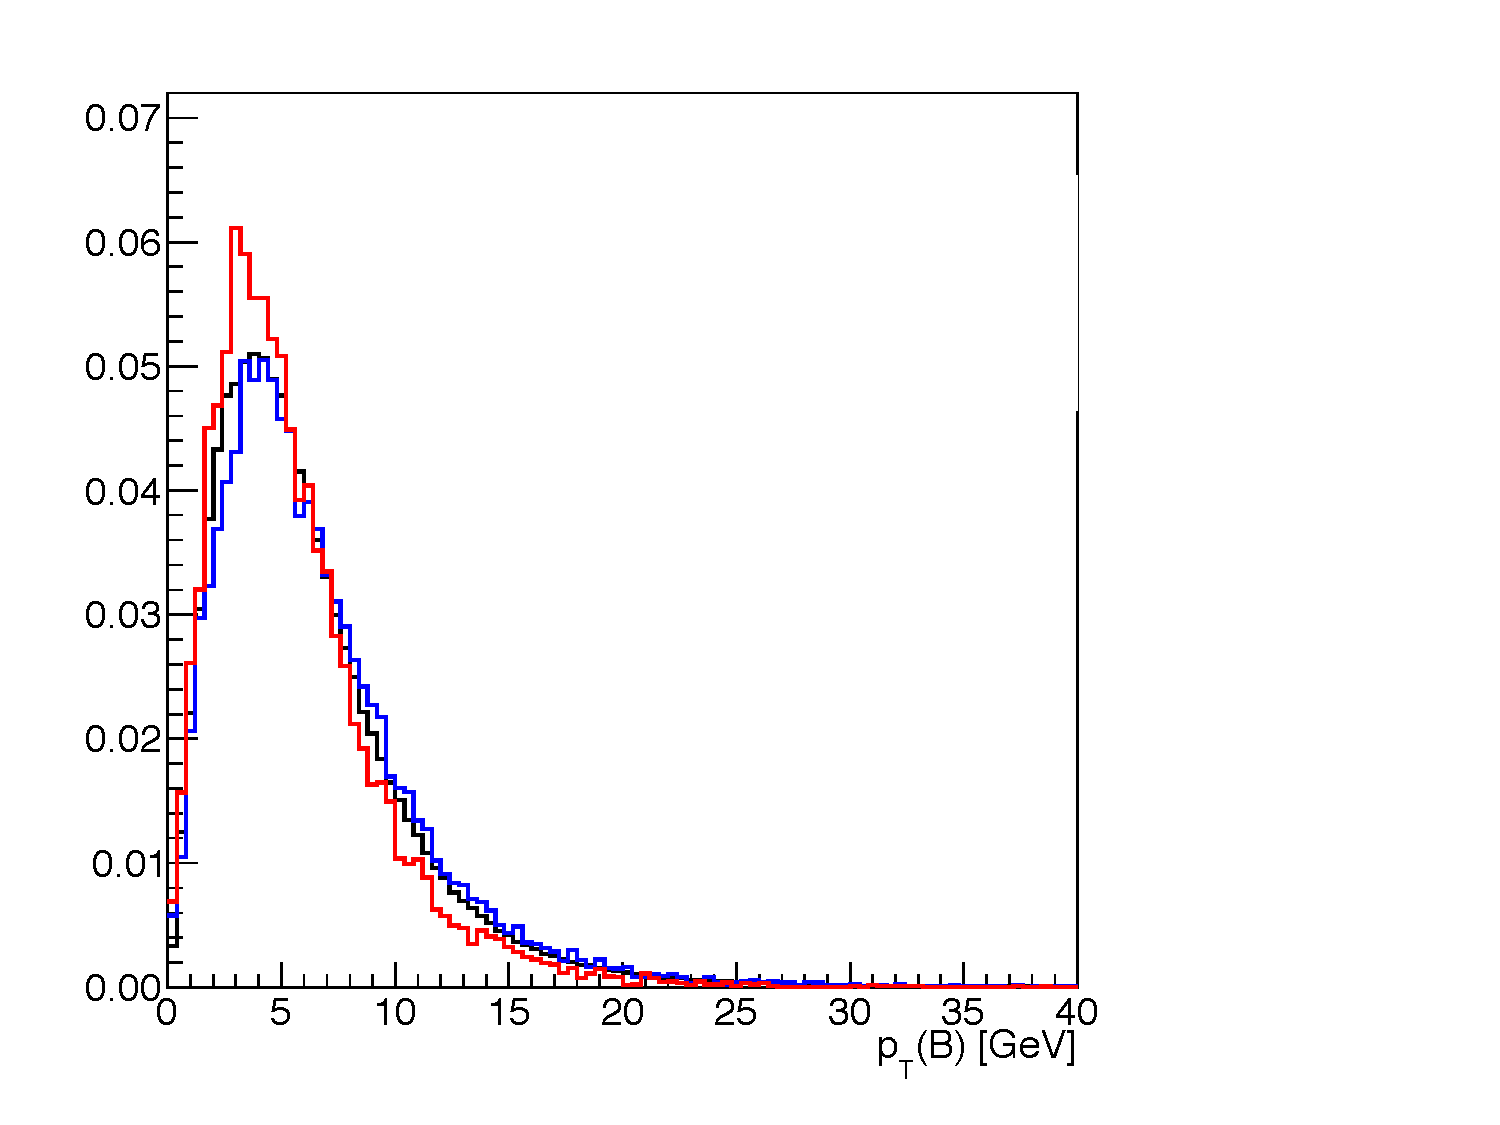
\includegraphics[width=0.31\textwidth]{private/content/flavour-tagging/figs/lhcb_ft_calibration_bu2jpsik_pT}
  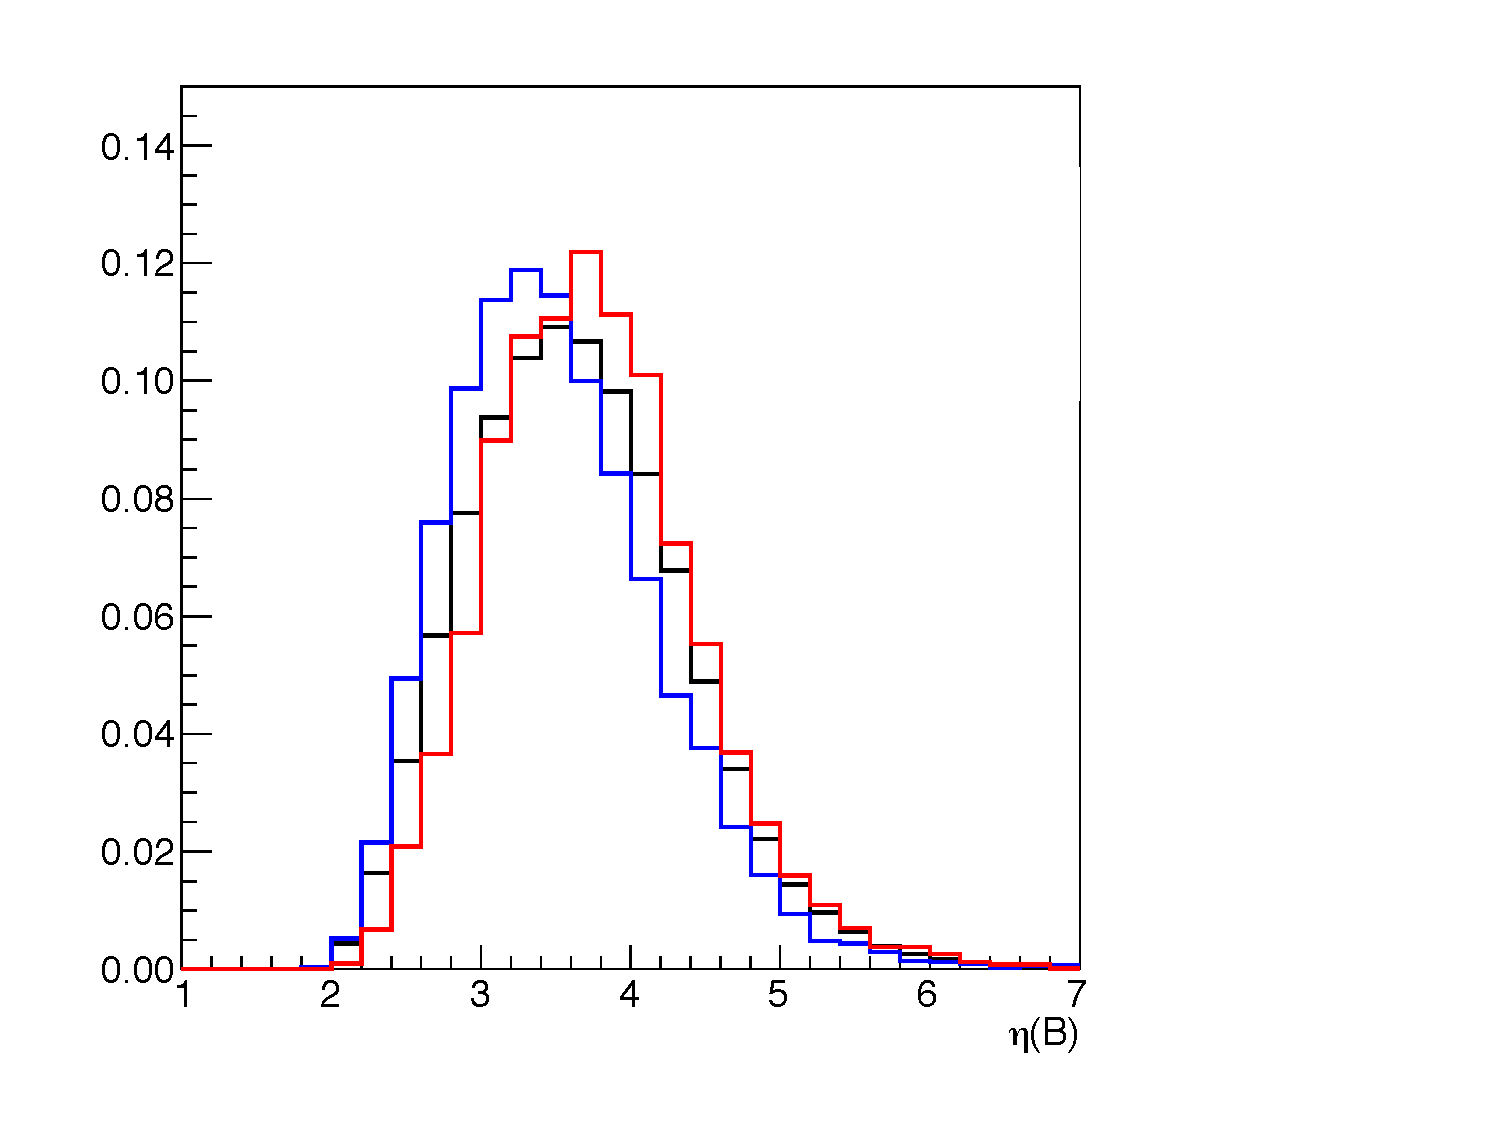
\includegraphics[width=0.31\textwidth]{private/content/flavour-tagging/figs/lhcb_ft_calibration_bu2jpsik_eta}
  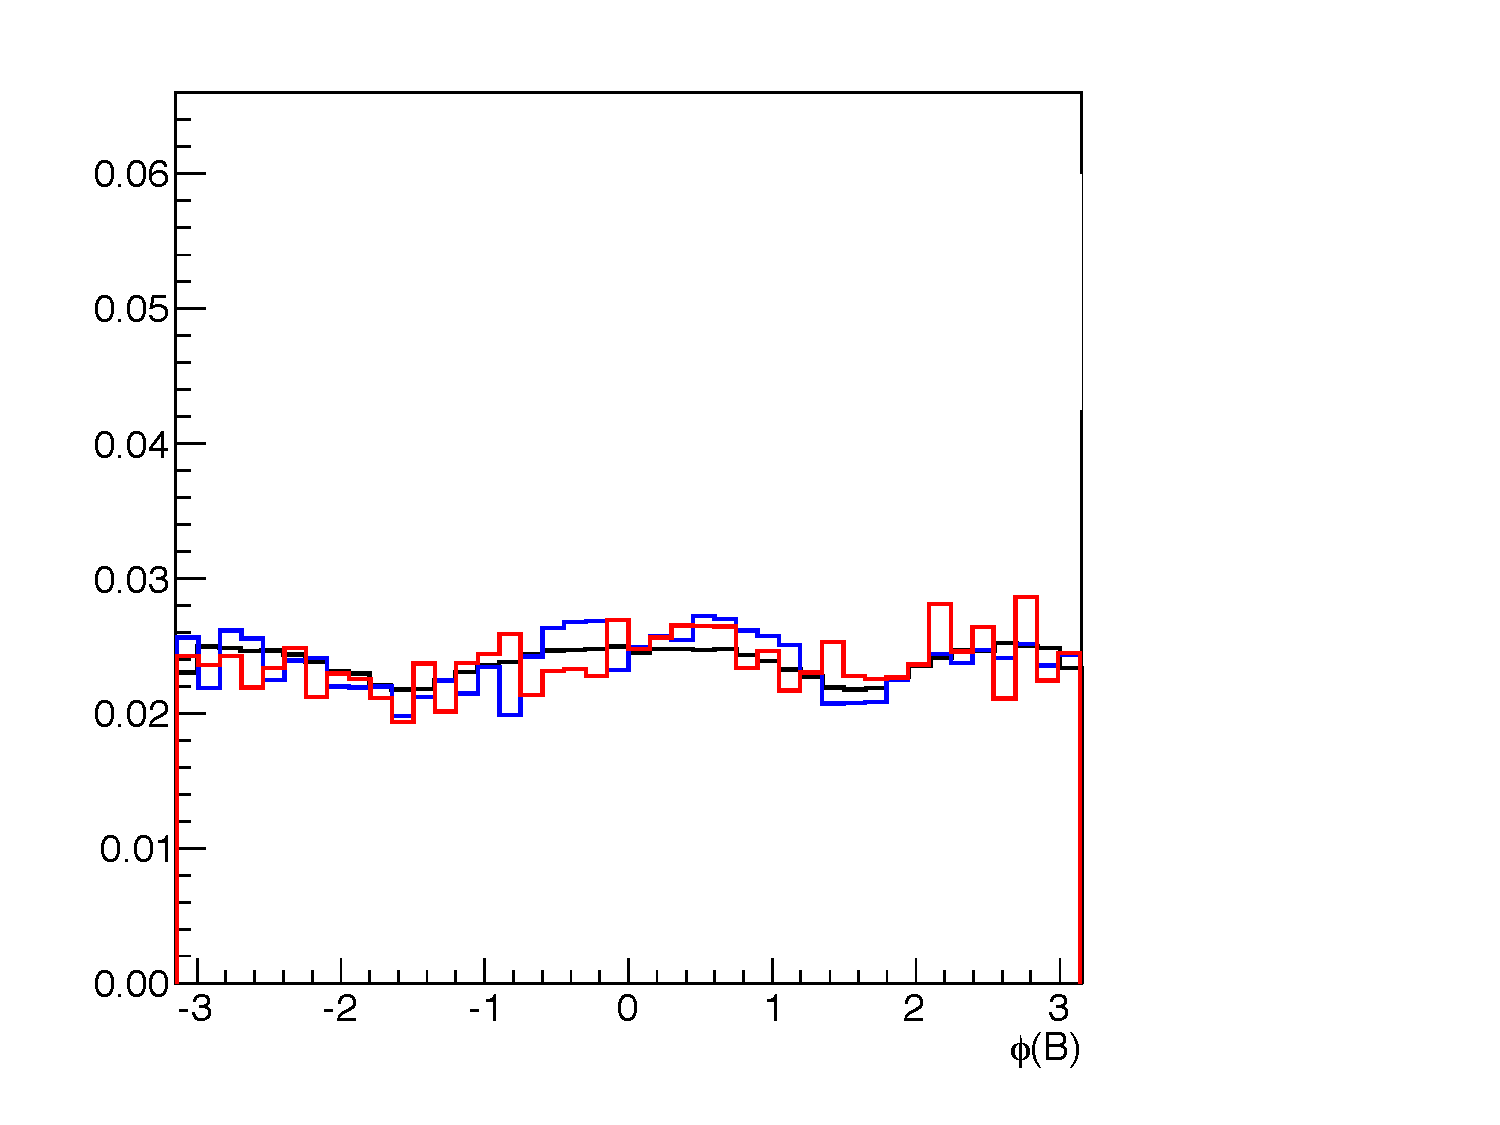
\includegraphics[width=0.31\textwidth]{private/content/flavour-tagging/figs/lhcb_ft_calibration_bu2jpsik_phi}
  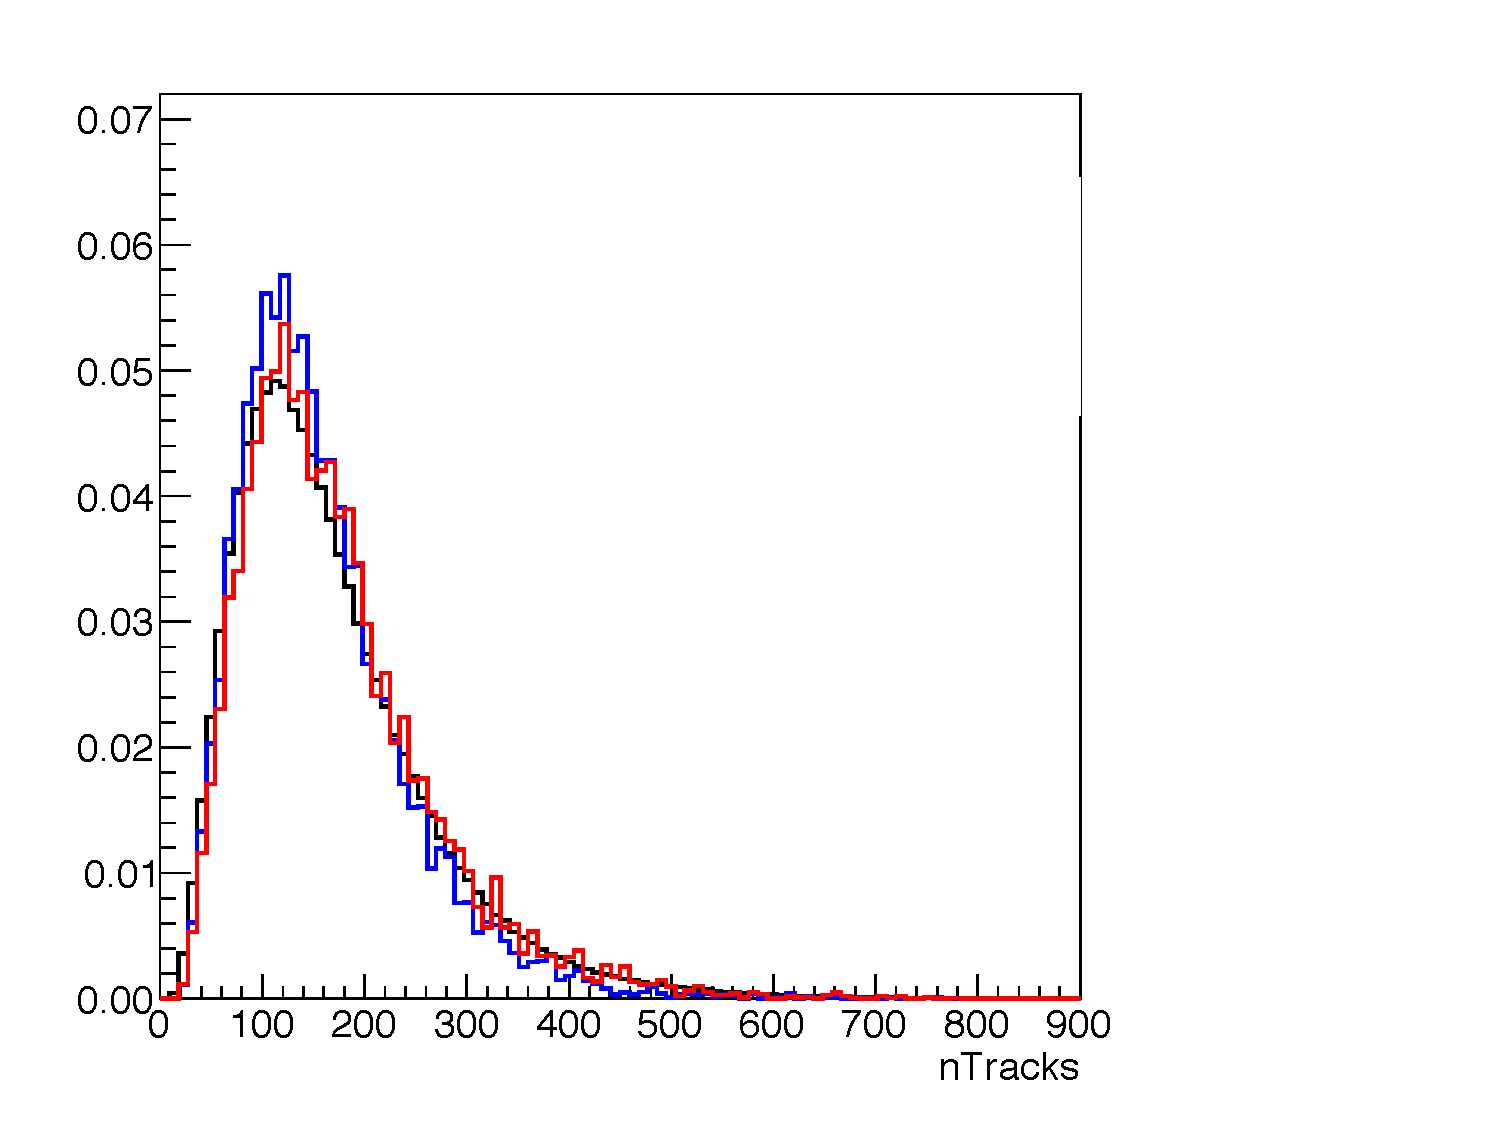
\includegraphics[width=0.31\textwidth]{private/content/flavour-tagging/figs/lhcb_ft_calibration_bu2jpsik_nTracks}
  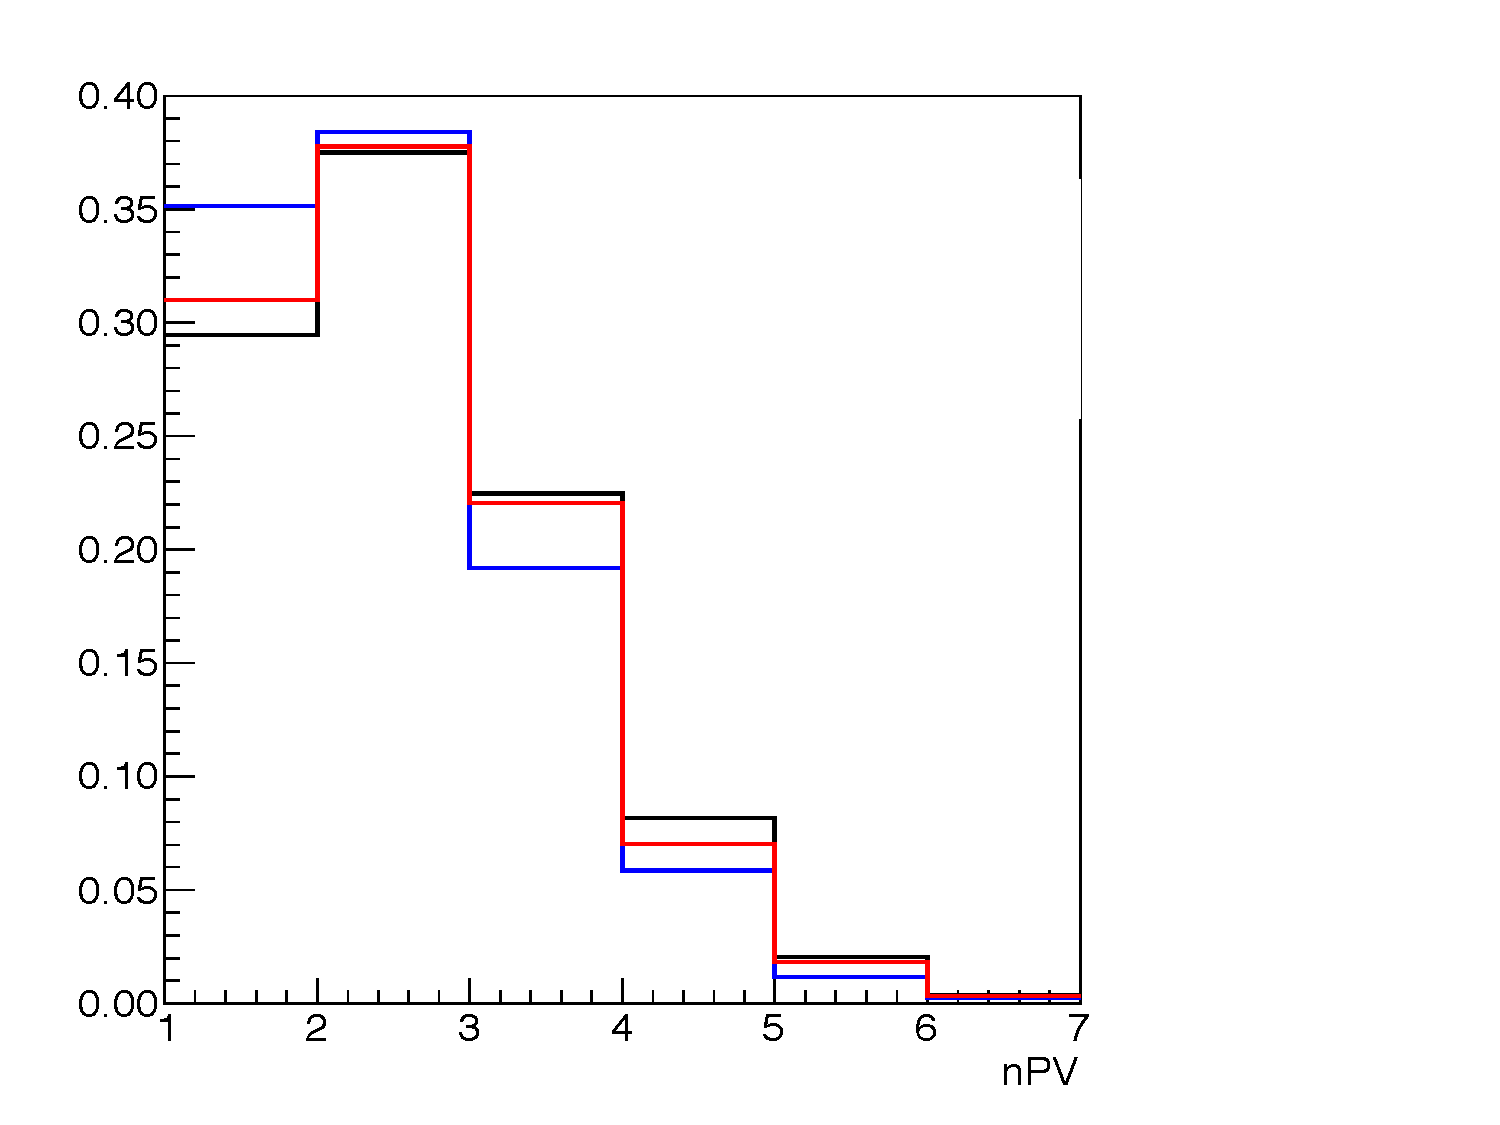
\includegraphics[width=0.31\textwidth]{private/content/flavour-tagging/figs/lhcb_ft_calibration_bu2jpsik_nPV}
  \caption{Weighted distributions of the \Bmeson \acf{pT}, \acf{pseudorapidity},
  and azimuthal angle ($\phi$), as well as the number of tracks (nTracks) and
  \aclp{PV} (n\acsp{PV}) in the event. In black the $\BuToJpsiK$ distributions
  are shown. $\BdToJpsiKS$ signal candidates belonging to the long track
  (downstream track) sub-sample contribute to the red (blue) histograms.
  \cite{FT:RunI} \todo{Decide if to remove plots}
  }
  \label{fig:flavour_tagging:calibration:os:parameter_distributions}
\end{figure}
%
\missing{Comparison of $\BuToJpsiK$ and $\BdToJpsiKstar$ on MC}

% ------------------------------------------------------------------------------
\subsection[
  head={\ac{SS} tagger calibration using \BdToJpsiKstar decays},
  tocentry={\ac{SS} tagger calibration using \BdToJpsiKstarHyperref decays}
]{\ac{SS} tagger calibration using \BdToJpsiKstarbfsf decays}
\label{sec:flavour_tagging:calibration:ss}

The \SSpi mistag estimate is pre-calibrated using the calibration parameters
%
\begin{equation}
\label{eq:tagging:sspion_precalibration}
    \p{0}{} = \num{0.425}\eqcm\eqspace
    \p{1}{} = \num{0.939}\eqcm\eqspace
    \langle\eta\rangle = \num{0.379}.
\end{equation}
%
Following, the \SSpi tagger is calibrated using a dataset of $\BdToJpsiKstar$
decays corresponding to an integrated luminosity of $\SI{3.0}{\per\fb}$
collected by the \LHCb experiment in \RunOne. As the \SSpi tagging algorithm
depends on the fragmentation process of the initial \Bmeson, a $\Bd$ decay mode
is preferred over a decay of $\Bu$ mesons. Only candidates carrying a tagging
response from the \SSpi tagger are considered in the following.
\missing{\SS calibration: $\BdToJpsiKstar$ signal selection?}

To describe the mixing asymmetry $\MixingAsymmetry$ a two-dimensional fit to the
reconstructed decay time and mass distribution is performed. The signal mass
component is described by an Ipatia \PDF (\cf
\cref{sec:measurement_of_sin2beta:likelihood_fit:pdfs:ipatia}) with all tail
parameters fixed to values determined on simulations. The description of the
combinatorial background component consists of a sum of two exponential
\acp{PDF} with shared parameters in the mass dimension to reflect two
background components with different lifetimes seen in the decay time dimension.
Hence, the background decay time distribution is modelled by two exponential
functions as well. The decay time signal \PDF contains an acceptance function
$\eps(t)$ describing reconstruction and selection inefficiencies for signal
candidates with low decay times and a convolution of a $\B$ mixing \PDF and a
resolution model
%
\begin{equation}
  \Prob{\Sig}{} = \eps(t) \cdot \left[ \Prob{\text{Mix}}{}(t, \tagdecision, \tagdecision^\prime, \mistagestimate) \otimes \mathcal{R}(t - t_\text{true}) \right] \eqcm
\end{equation}
%
with
%
\begin{equation}
  \Prob{\text{Mix}}{}(t, \tagdecision, \tagdecision^\prime, \mistagestimate) 
  \propto 
  \exponential{-\sfrac{t}{\tau}} \left( 1 - \tagdecision \Delta\mistag + \tagdecision \tagdecision^\prime (1 - 2 \langle\mistag\rangle) \cos(\DMd t) \right)\eqcm
\end{equation}
%
where the acceptance function is parametrised as
%
\begin{equation}
  \eps(t) = \arctan(t \exponential{\alpha t+ \beta})\eqpd
\end{equation}
%
The resolution model consists of a single Gaussian resolution function
$\mathcal{R}(t - t_\text{true})$ with the width fixed to
$\SI{50}{\femto\second}$ and no offset from zero. The parameters $\alpha$ and
$\beta$ of the acceptance function are fixed in the fit to values determined on
simulated candidates. The mixing \PDF depends on the decay time $t$, the tag
decision $\tagdecision$ of the \SSpi tagging algorithm, and the tag
$\tagdecision^\prime$ extracted from the final state flavour (\cf
\cref{eq:flavour_tagging:calibration:method:charged:tagdefinition}). This
parametrisation includes the mistag difference $\deltamistag$ and the arithmetic
average of the mistag $\langle\mistag\rangle$ for the given dataset and
therefore no per-event mistag information enter the fit model. To strike a
balance between the per-event technique outlined in
\cref{sec:flavour_tagging:calibration:method} and complexity of the fit model,
an intermediate approach is chosen. The calibration is performed by a
simultaneous fit in $\num{5}$ equally filled bins of the mistag estimate
$\mistagestimate$. The per-bin average $\langle\mistagestimate\rangle_i$ of all
signal candidates is computed using the \splot method \cite{Pivk:2004ty}. Then,
the calibration can be parametrised inside the \PDF
%
\begin{equation}
  \begin{split}
    \Delta\mistag         &= \deltapzero + \deltapone ( \langle\mistagestimate\rangle_i - \langle\mistagestimate\rangle )\eqcm \\
    \langle\mistag\rangle &= \pzero + \pone ( \langle\mistagestimate\rangle_i - \langle\mistagestimate\rangle )\eqcm
  \end{split}
\end{equation}
%
with the calibration parameters $\pzero$, $\pone$, $\deltapzero$, and
$\deltapone$ are shared among all sub-samples of data where
$\langle\mistagestimate\rangle$ and $\langle\mistagestimate\rangle_i$ denote the
average mistag estimates for the total dataset and the correspondent
sub-samples. \Cref{fig:flavour_tagging:calibration:ss:fit} presents the mass and
decay time distributions of the $\BdToJpsiKstar$ candidates, as well as
projections of the fitted \PDF components. The calibration parameters are
determined to be
%
\begin{equation}\label{eq:flavour_tagging:calibration:ss:parameters}
  \begin{split}
    \p{0}{\text{\acs{SSpi}}}        &= \phantom{+}0.4232 \pm\, 
                                       0.0029 \text{\,(\stat)} \pm\, 
                                       0.0020 \text{\,(\syst type I)} \pm\, 
                                       0.0019 \text{\,(\syst type II)} \eqcm\\ % 0.0040 syst
    \p{1}{\text{\acs{SSpi}}}        &= \phantom{+}1.011\phantom{0} \pm\, 
                                       0.064\phantom{0} \text{\,(\stat)} \pm\, 
                                       0.009\phantom{0} \text{\,(\syst type I)} \pm\, 
                                       0.030\phantom{0} \text{\,(\syst type II)} \eqcm\\ % 0.034 syst
    \deltap{0}{\text{\acs{SSpi}}} &= -0.0026 \pm\, 
                                      0.0043 \text{\,(\stat)} \pm\, 
                                      0.0024 \text{\,(\syst type I)} \pm\, 
                                      0.0013 \text{\,(\syst type II)} \eqcm \\
    \deltap{1}{\text{\acs{SSpi}}} &= -0.171\phantom{0} \pm\, 
                                      0.096\phantom{0} \text{\,(\stat)} \pm\, 
                                      0.029\phantom{0} \text{\,(\syst type I)} \pm\, 
                                      0.027\phantom{0} \text{\,(\syst type II)} \eqcm\text{ and} \\
    \langle\mistagestimate^{\text{\acs{SSpi}}}\rangle &= \phantom{+}0.425 \eqcm
  \end{split}
\end{equation}
%
and the inter-parameter correlations are given in
\cref{tab:flavour_tagging:calibration:ss:correlations}.
%
\begin{table}
  \centering
  \caption{Correlations between the \SSpi tagging calibration parameters.}
  \label{tab:flavour_tagging:calibration:ss:correlations}
  \begin{tabular}{ccccc}
    \toprule
    & $\p{0}{\text{\acs{SSpi}}}$ & $\p{1}{\text{\acs{SSpi}}}$ & $\deltap{0}{\text{\acs{SSpi}}}$ & $\deltap{1}{\text{\acs{SSpi}}}$ \\
    \midrule
    $\p{0}{\text{\acs{SSpi}}}$ & 1 & 0.04 & -0.007 & 0.0004 \\
    $\p{1}{\text{\acs{SSpi}}}$ & 0.04 & 1 & 0.0016 & -0.006 \\
    $\deltap{0}{\text{\acs{SSpi}}}$ & -0.007 & 0.0016 & 1 & 0.03 \\
    $\deltap{1}{\text{\acs{SSpi}}}$ & 0.0004 & -0.006 & 0.03 & 1 \\
    \bottomrule
  \end{tabular}
\end{table}
%
\begin{figure}[t]
  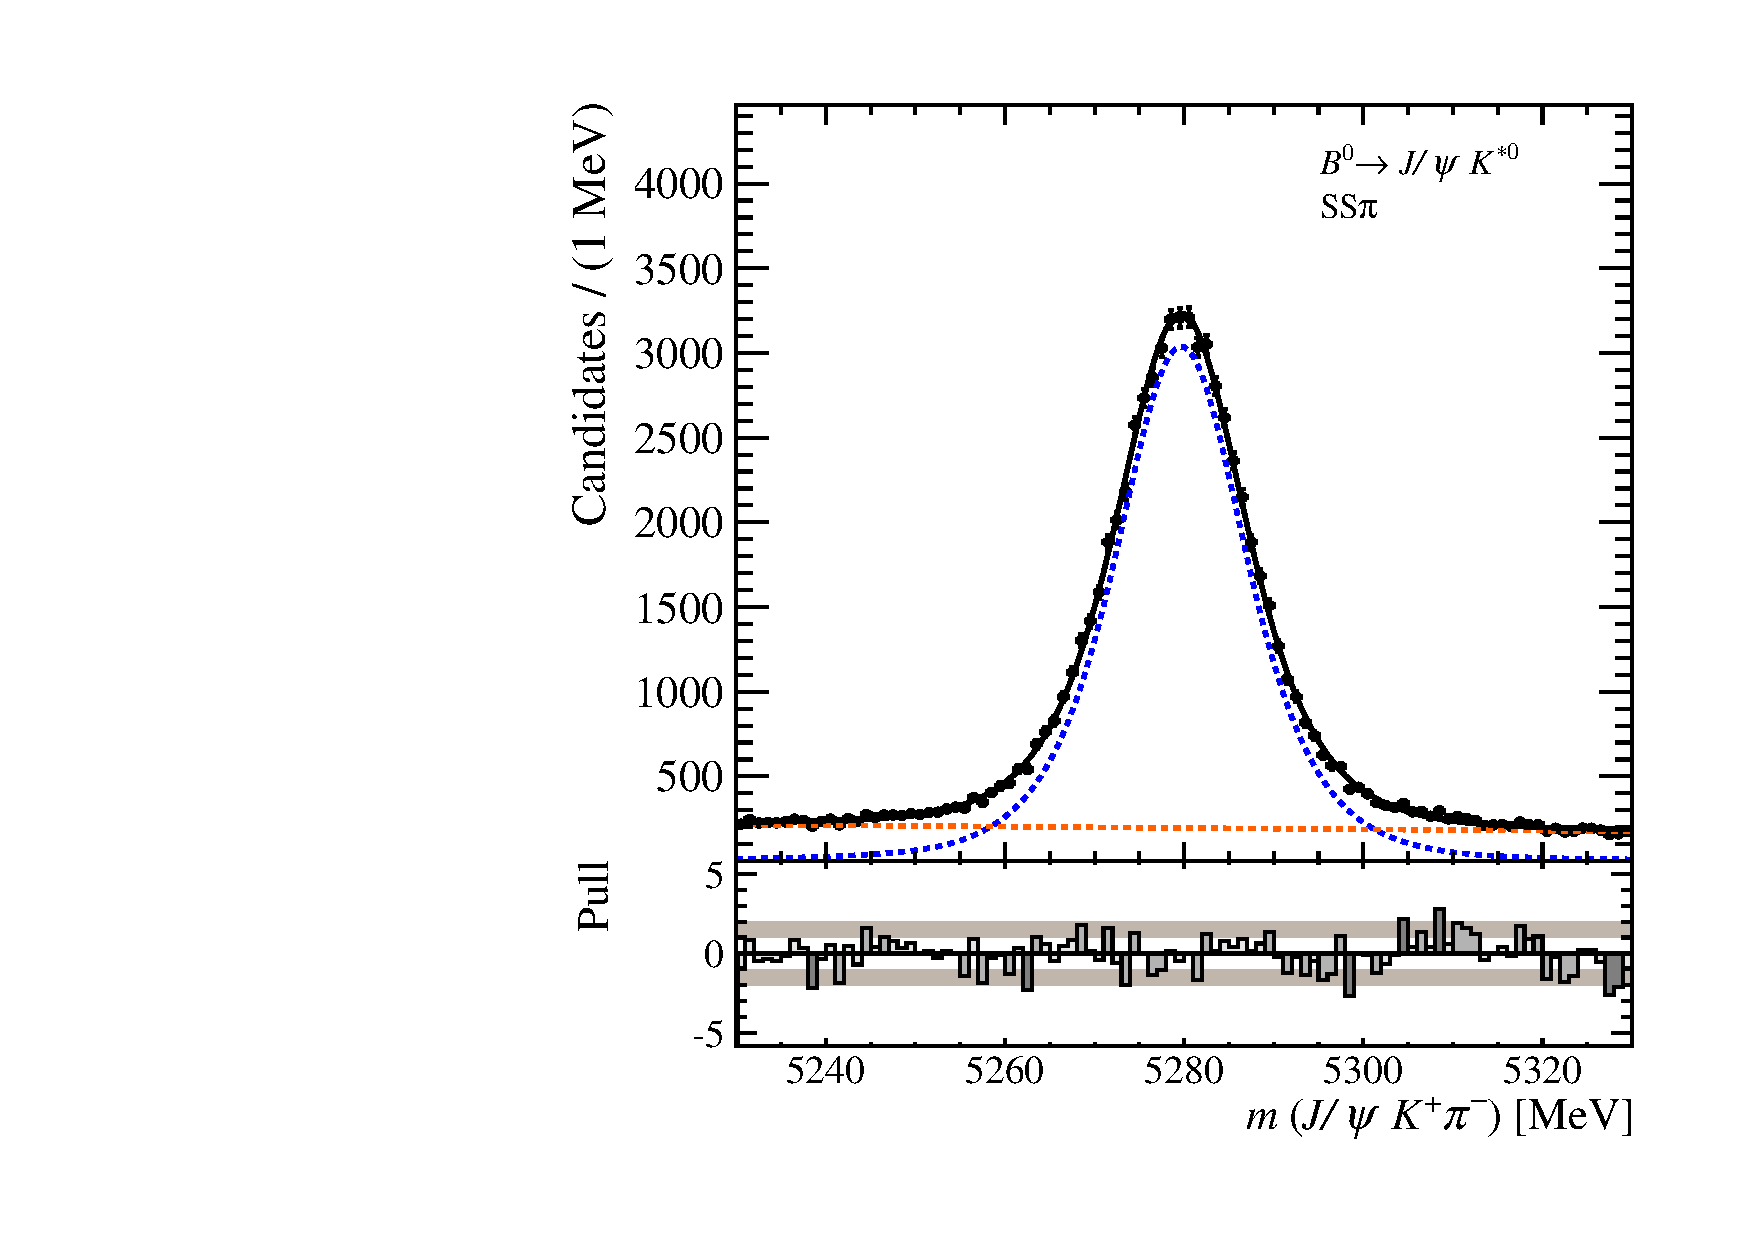
\includegraphics[width=0.48\textwidth]{private/content/flavour-tagging/figs/lhcb_ft_calibration_bd2jpsikstar_mass.pdf}
  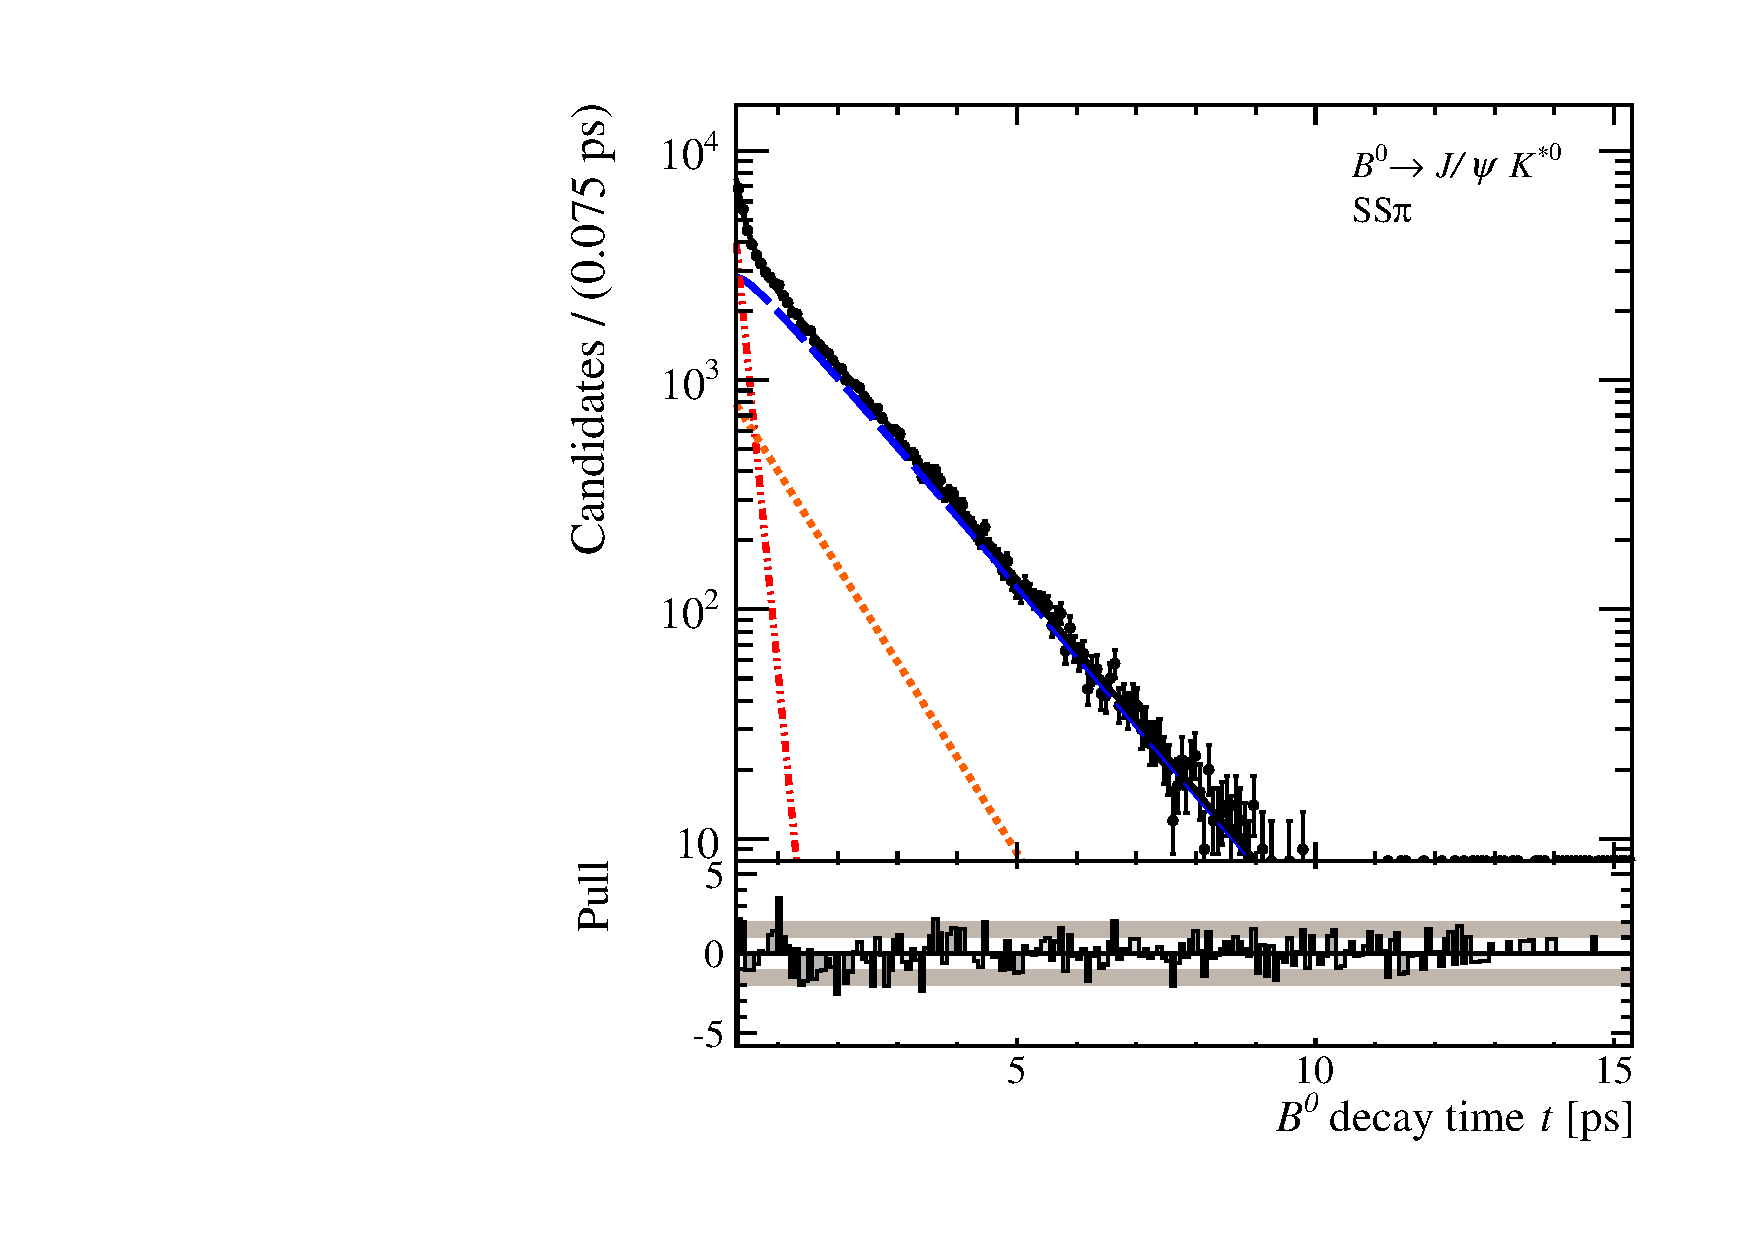
\includegraphics[width=0.48\textwidth]{private/content/flavour-tagging/figs/lhcb_ft_calibration_bd2jpsikstar_time.pdf}
  \caption{(Left) Mass and (Right) decay time distributions of $\BdToJpsiKstar$
  candidates. In blue the projections of the fitted signal components and in
  red/orange the projections of the combinatorial background component are
  shown. \cite{FT:RunI}}
  \label{fig:flavour_tagging:calibration:ss:fit}
\end{figure}
%
The type I systematic uncertainties cover influences of the decay time
acceptance and resolution, the production and detection asymmetries, as well as
possible deviations of the results when performing a fit using a signal
\sweighted dataset. The study of the type II systematic uncertainties follows
closely the approach outlined in \cref{sec:flavour_tagging:os}. A comparison of
the parameter distributions between the calibration and the signal channel is
given in \cref{fig:flavour_tagging:calibration:ss:parameter_distributions}, the
results of the reweighting procedure are presented in
\cref{tab:flavour_tagging:calibration:ss:systematics}.
%
\begin{table}
  \centering
  \caption{Summary of type II systematic uncertainties for \SSpi calibration
  parameters.}
  \label{tab:flavour_tagging:calibration:ss:systematics}
  \begin{tabular}{ccccc}
    \toprule
      & $\delta\pzero$ & $\delta\pone$ & $\delta\deltapzero$ & $\delta\deltapone$ \\
      & $(10^{-3})$    & $(10^{-2})$   & $(10^{-3})$         & $(10^{-2})$        \\
    \midrule
    $\text{\acs{pT}}$             & 1.3  & 2.1   & 0.6  & 2.7  \\
    $\text{\acs{pseudorapidity}}$ & 0.23 & 0.020 & 0.7  & 0.5  \\
    $\phi$                        & 0    & 0.6   & 0.14 & 0.27 \\
    nTracks                       & 1.5  & 2.0   & 1.1  & 0.08 \\
    nPVs                          & 0.6  & 0.5   & 0    & 0.05 \\
    \midrule
      Total                       & 1.9  & 3.0   & 1.3  & 2.7 \\
    \midrule
    Percentage of & 
    \multirow{2}[2]{*}{\SI{65.5}{\percent}} & 
    \multirow{2}[2]{*}{\SI{46.9}{\percent}} & 
    \multirow{2}[2]{*}{\SI{30.2}{\percent}} & 
    \multirow{2}[2]{*}{\SI{28.1}{\percent}} \\
    stat. uncert. \\
    \bottomrule
  \end{tabular}
\end{table}
%
\begin{figure}
  \centering
  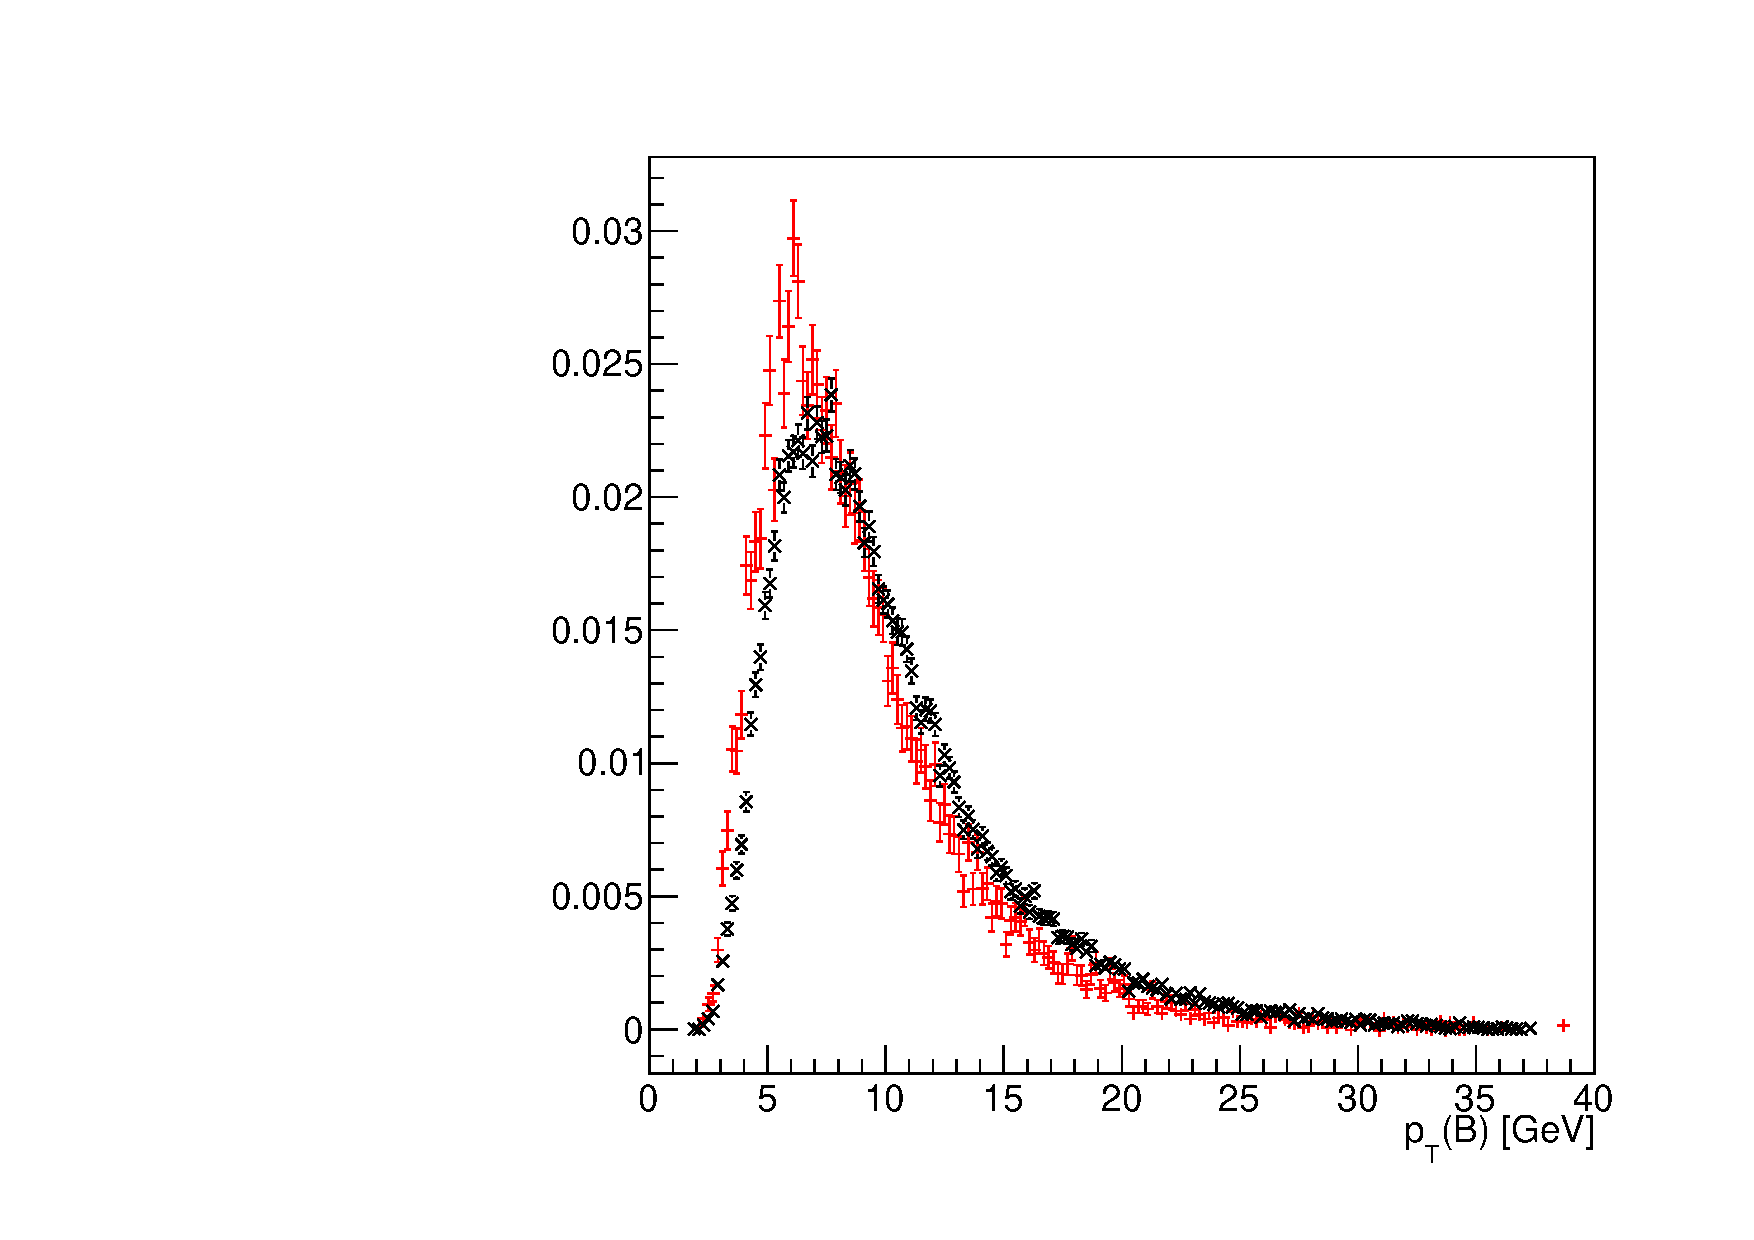
\includegraphics[width=0.31\textwidth]{private/content/flavour-tagging/figs/lhcb_ft_calibration_bd2jpsikstar_pT}
  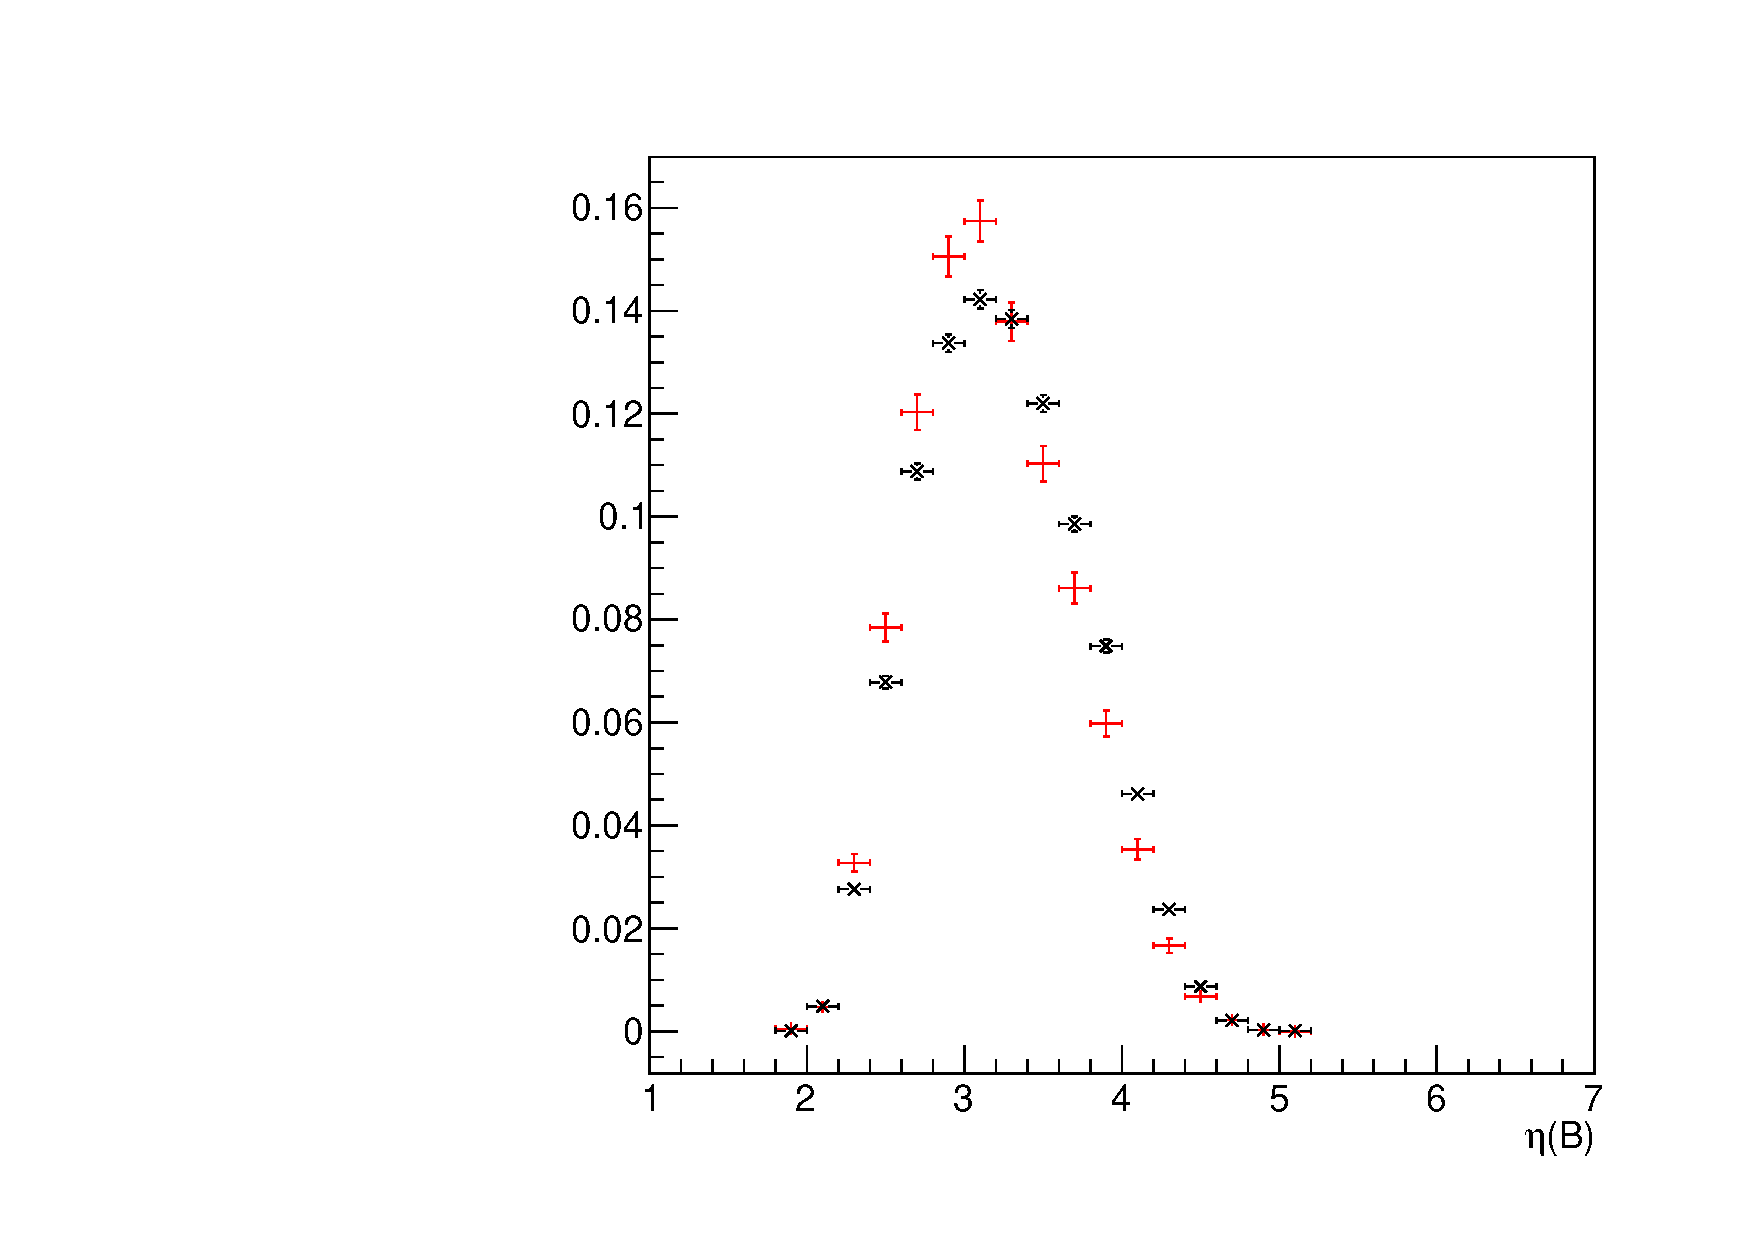
\includegraphics[width=0.31\textwidth]{private/content/flavour-tagging/figs/lhcb_ft_calibration_bd2jpsikstar_eta}
  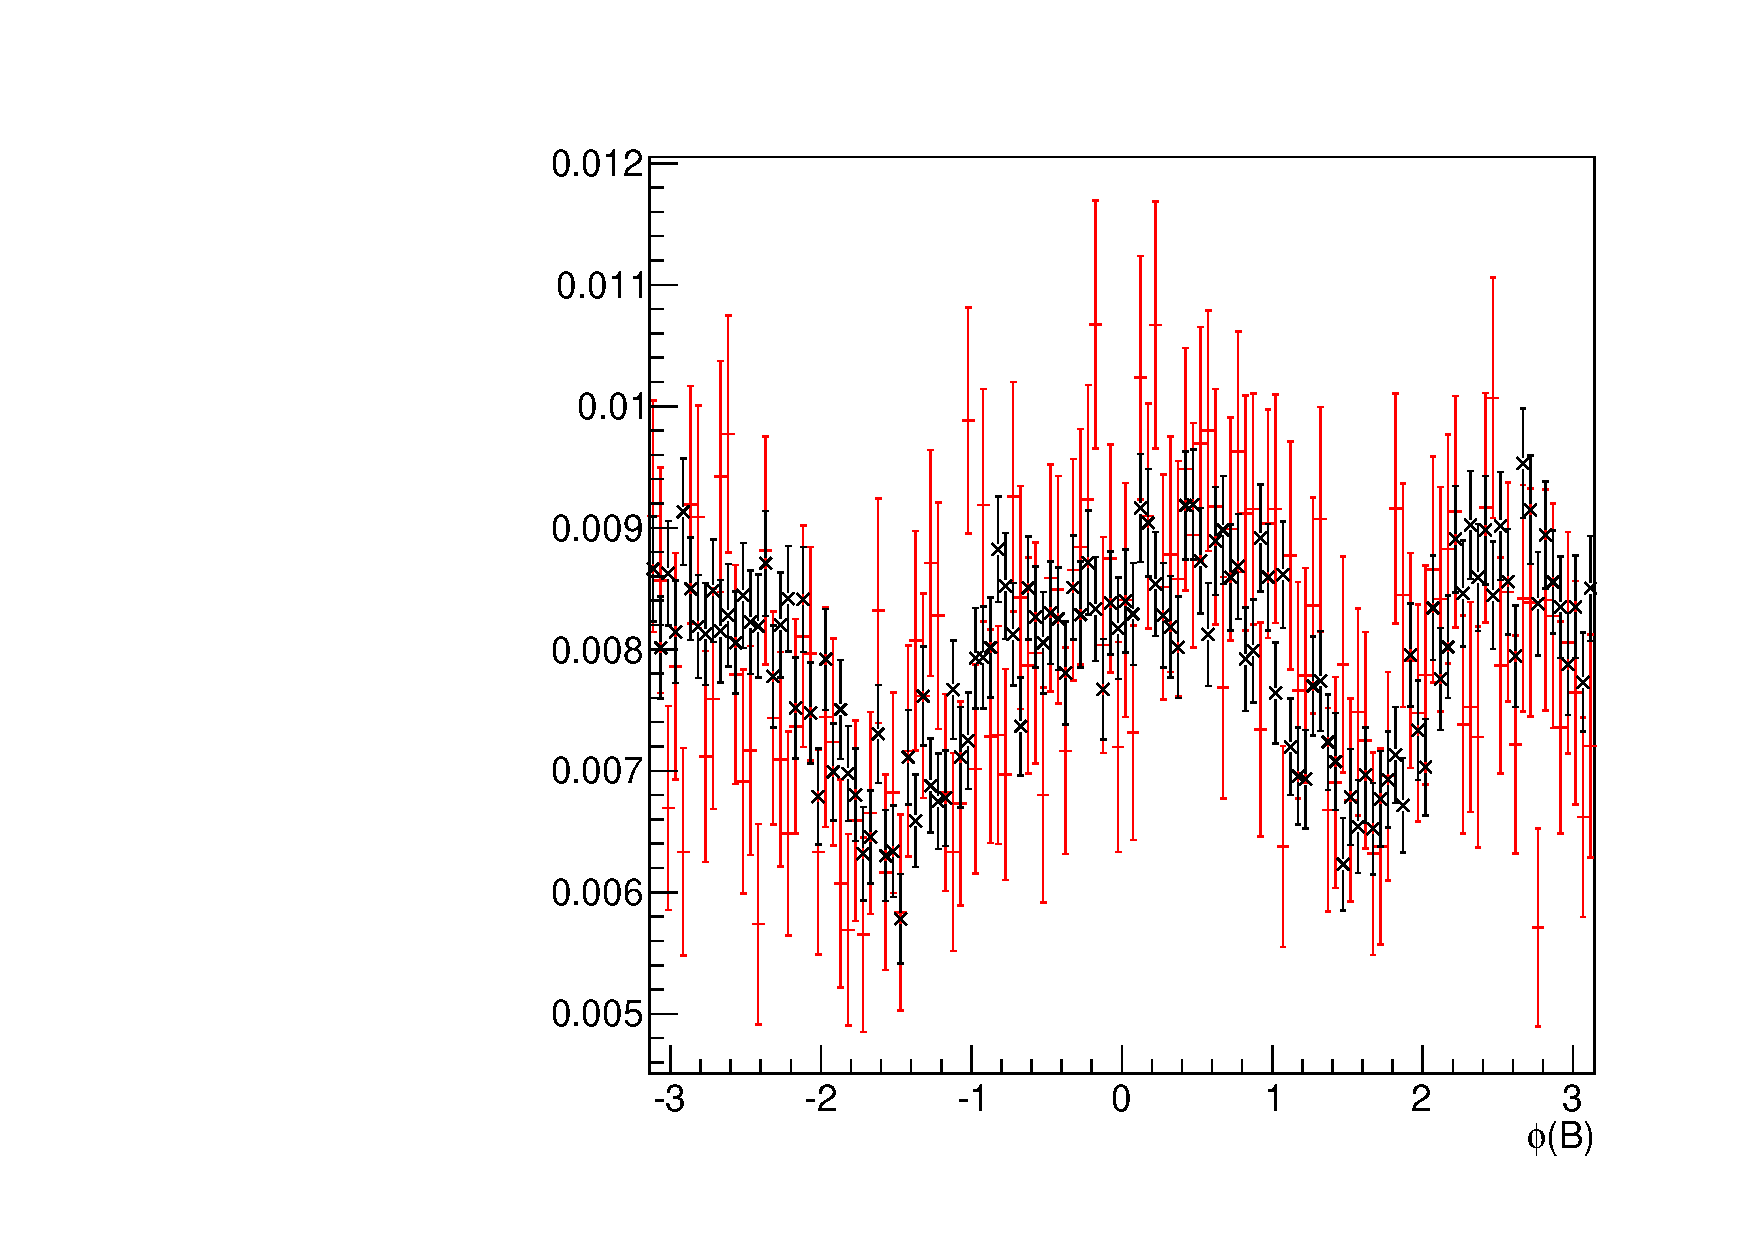
\includegraphics[width=0.31\textwidth]{private/content/flavour-tagging/figs/lhcb_ft_calibration_bd2jpsikstar_phi}
  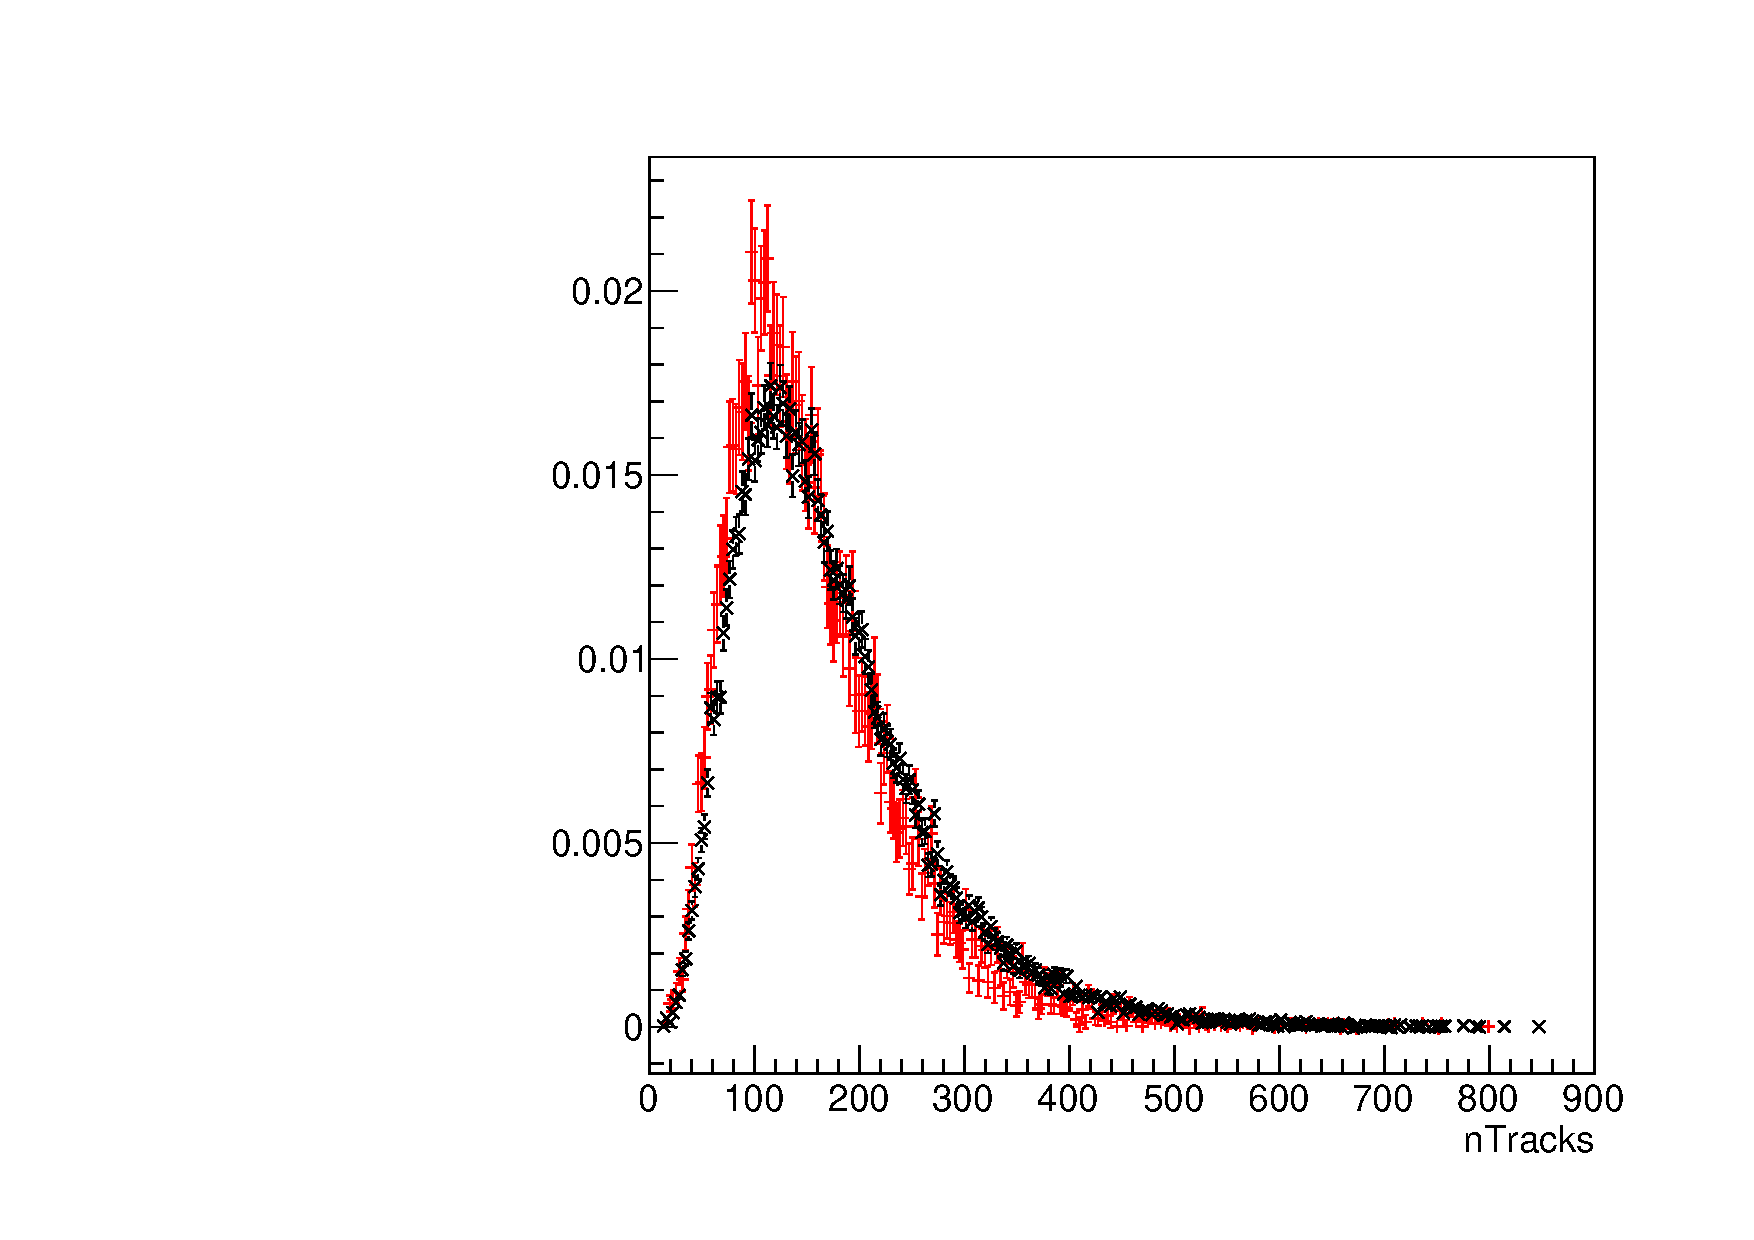
\includegraphics[width=0.31\textwidth]{private/content/flavour-tagging/figs/lhcb_ft_calibration_bd2jpsikstar_nTracks}
  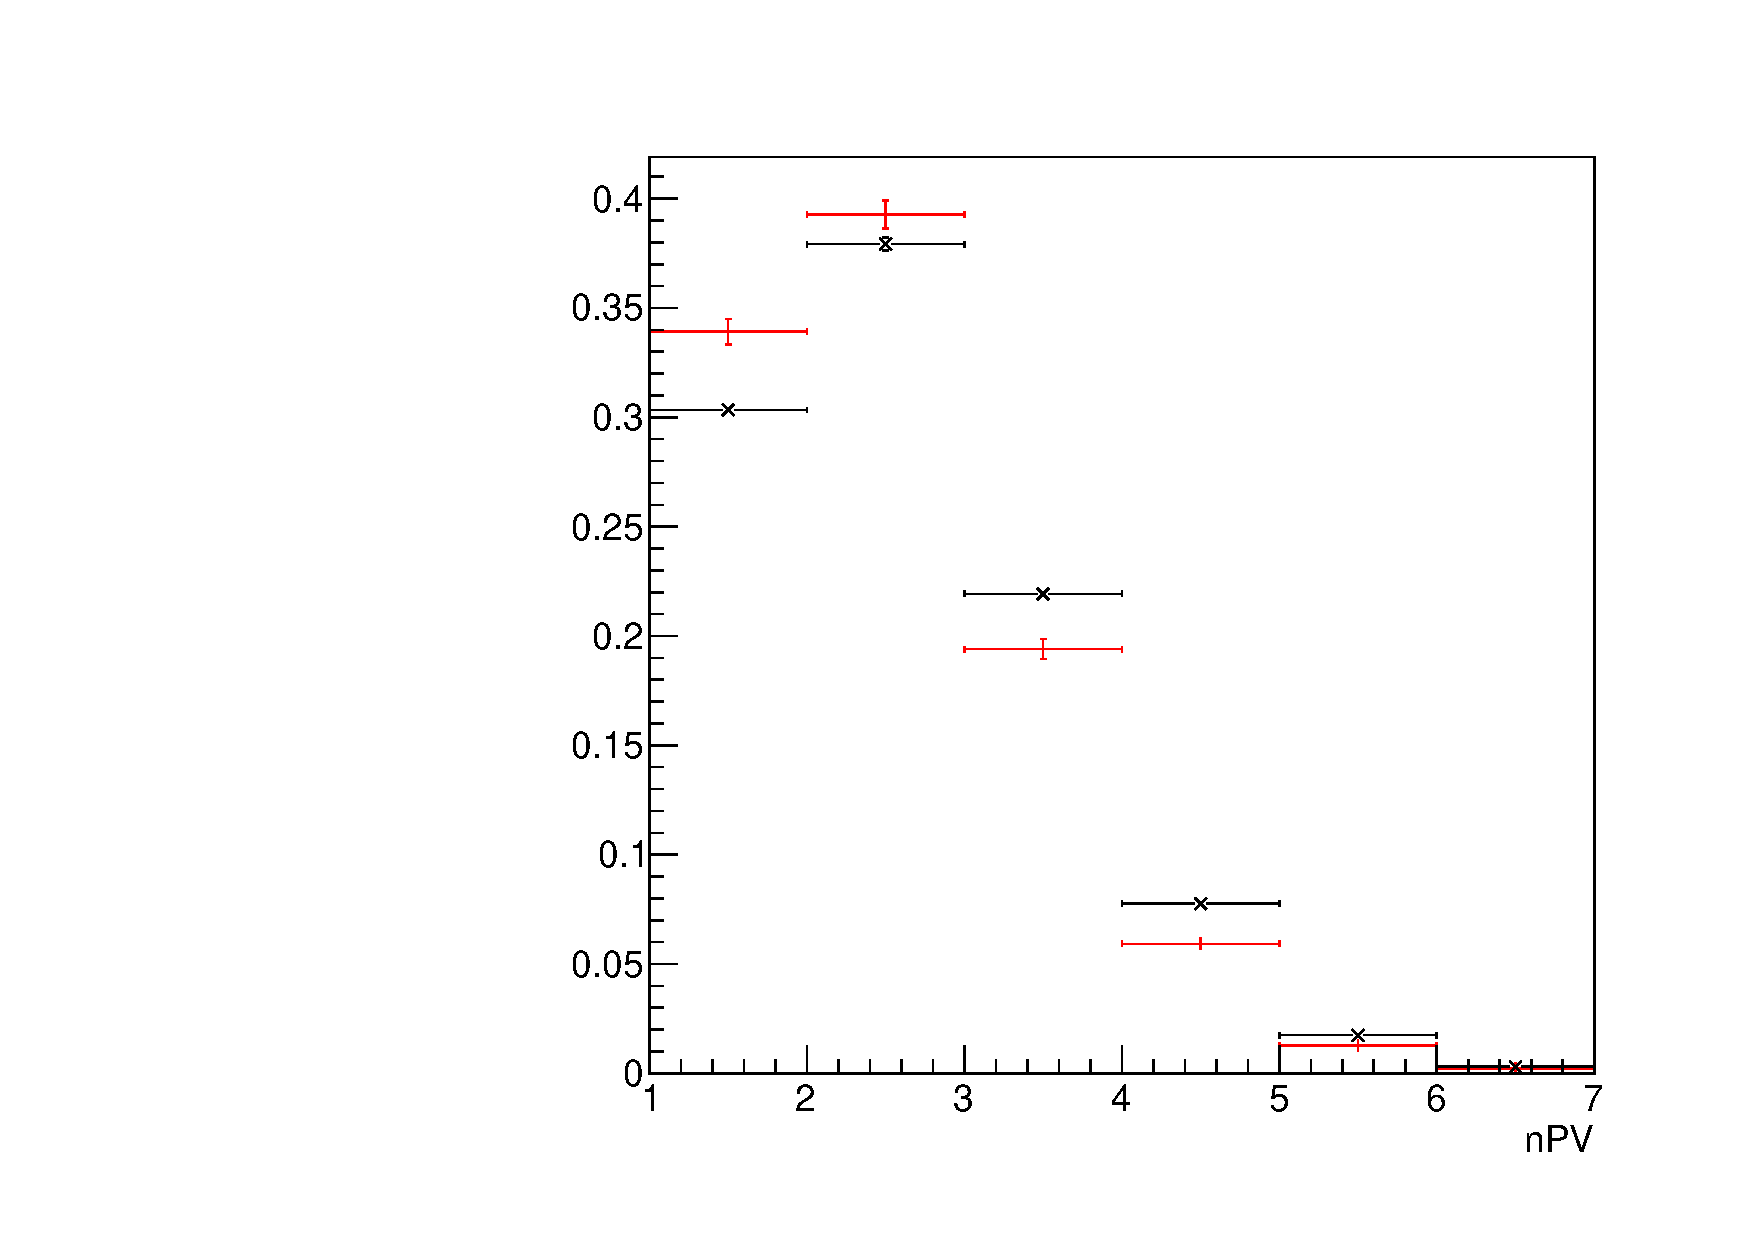
\includegraphics[width=0.31\textwidth]{private/content/flavour-tagging/figs/lhcb_ft_calibration_bd2jpsikstar_nPV}
  \caption{Weighted distributions of the \Bmeson \ac{pT}, \ac{pseudorapidity},
  and azimuthal angle, as well as the number of tracks and \aclp{PV} in the
  event. The comparisons show the distributions for (red) $\BdToJpsiKS$ and
  (black) $\BdToJpsiKstar$ candidates.
  \cite{FT:RunI}\todo{Decide if to remove plots}
  }
  \label{fig:flavour_tagging:calibration:ss:parameter_distributions}
\end{figure}

% %%%%%%%%%%%%%%%%%%%%%%%%%%%%%%%%%%%%%%%%%%%%%%%%%%%%%%%%%%%%%%%%%%%%%%%%%%%%%%
\section{Combination of single tagger outputs}
\label{sec:flavour_tagging:combination}

In order to fully exploit the information of all tagging algorithms it is
desirable to combine their tag decisions $\tagdecision_i$ and mistag estimates
$\mistagestimate_i$ into one mutual decision. Given the probabilities
$p(\bquark)$ and $p(\bquarkbar)$ that a meson contains either a $\bquark$ or a
$\bquarkbar$ quark
%
\begin{equation}\label{eq:flavour_tagging:combination:product}
  \begin{split}
    p(\bquark)    &= \prod_i\left( \frac{1 + \tagdecision_i}{2} - \tagdecision_i (1 - \mistagestimate_i) \right)\eqcm\\
    p(\bquarkbar) &= \prod_i\left( \frac{1 - \tagdecision_i}{2} + \tagdecision_i (1 - \mistagestimate_i) \right)\eqcm
  \end{split}
\end{equation}
%
the combined probabilities $P(\bquark)$ and $P(\bquarkbar)$ can be calculated
%
\begin{equation}\label{eq:flavour_tagging:combination:total}
  P(\bquark)    = \frac{p(\bquark)}{p(\bquark) + p(\bquarkbar)}\eqcm\eqspace
  P(\bquarkbar) = 1 - P(\bquark)\eqpd
\end{equation}
%
Then, the combined tag decision and mistag estimate are $\tagdecision = +1$ and
$\mistagestimate = 1 - P(\bquarkbar)$ if $P(\bquarkbar) > P(\bquark)$, otherwise
$\tagdecision = -1$ and $\mistagestimate = 1 - P(\bquark)$. As
\cref{eq:flavour_tagging:combination:product} ignores possible correlation among
the involved taggers, the joint mistag estimate might distort the outcome. To
correct for this bias the combination is calibrated using a flavour-specific
control channel.

The analysis presented in this thesis utilises the combination of the calibrated
\OS tagging algorithms (see \cref{sec:flavour_tagging:calibration:os}) as well
as of the \SSpi tagger (see \cref{sec:flavour_tagging:calibration:ss}). As the
\OS and \SS taggers find their decisions using independent particle information
their output is assumed to be uncorrelated and not further calibration is
necessary after combining the \OS and \SSpi tagging decisions.

% %%%%%%%%%%%%%%%%%%%%%%%%%%%%%%%%%%%%%%%%%%%%%%%%%%%%%%%%%%%%%%%%%%%%%%%%%%%%%%
\section{Performance}
\label{sec:flavour_tagging:performance}

The effective tagging efficiency (\cf \cref{eq:flavour_tagging:efftageff})
inherent in the used data sample given the choice of utilised taggers is
calculated as the sum of the effective tagging efficiencies carried by each
(including untagged) signal candidate
%
\begin{equation}
  \efftageff = \frac{\sum_{i=0}^{N} \mistag_i \tagdilution_i^2\big(\tagOS, \tagSS, \mistagOS, \mistagSS \big)}{\sum_{i=0}^{N} \mistag_i}\eqcm
\end{equation}
%
where $\mistagOS$ and $\mistagSS$ refer to the calibrated mistag estimates. This
adds up to an effective tagging efficiency of $\efftageff = \SI{3.02 +-
0.05}{\percent}$, which splits into a tagging efficiency of $\tageff = \SI{36.54
+- 0.14}{\percent}$ and an effective dilution of $\tagdilution = \SI{28.75 +-
0.24}{\percent}$ corresponding to an average mistag probability of $\mistag =
\SI{35.62 +- 0.12}{\percent}$.

\Cref{tab:flavour_tagging:performance:numbers} lists the tagging efficiency
separate for the tagging categories \catOS, \catSS, and \catBS, as well as for
the case where all \SSpi decisions are ignored and only the \OS tagging
information are exploited (\enquote{all \OS}) and vice versa (\enquote{all
\SSpi}). This allows the performance obtained on the given dataset to be
compared with the results from a previous \LHCb measurement \cite{Aaij:1497268},
where only the tagging information provided by the \OS algorithm were used.
Here, relative improvements of $\SI{10}{\percent}$ from $\SI{2.38}{\percent}$ to
$\SI{2.63}{\percent}$ can be observed. Finally, supplementing the measurement
with information from the \SSpi tagger allows for an overall improvement in
effective tagging efficiency of almost $\SI{27}{\percent}$.
%
\begin{table}
  \centering
  \caption{Effective tagging efficiency given for all three tagging categories.
  Additionally listed are the results just exploiting the information of the \OS
  or \SSpi tagging algorithms, as well as the total effective tagging efficiency
  of the dataset.}
  \label{tab:flavour_tagging:performance:numbers}
  \begin{tabular}{
      S[table-text-alignment = left]
      S
      [
        table-number-alignment = center,
        table-align-uncertainty = true,
        table-figures-decimal = 3,
        table-figures-uncertainty = 1,
      ]
    }
    \toprule
    {Tagger}        & {\efftageff [$\%$]}\\
    \midrule
    {\catOS}        & 2.259 +- 0.034 \\
    {\catSS}        & 0.262 +- 0.017 \\
    {\catBS}        & 0.503 +- 0.010 \\
    \midrule
    {all \OS}       & 2.63  +- 0.04  \\
    {all \SSpi}     & 0.376 +- 0.024 \\
    \midrule
    {Total}         & 3.02  +- 0.05  \\
    \bottomrule
  \end{tabular}
\end{table}
% 

% %%%%%%%%%%%%%%%%%%%%%%%%%%%%%%%%%%%%%%%%%%%%%%%%%%%%%%%%%%%%%%%%%%%%%%%%%%%%%%
\section{Recent developments and \RunTwo}
\label{sec:flavour_tagging:developments}

The algorithms utilised in the flavour tagging are always subject of active
development with the aim to improve their performance and gain new insights.
Several taggers are being revisited using particle selections based on
\acfp{ANN} or \acfp{BDT}.

% SSpi BDT
A \BDT based \SSpi tagging algorithm (\acs{BDTSSpi}) is in the stage of early
development, intended to replace the existing cut-based \SSpi tagger in the
future.

% OS and SS K NNet
% https://twiki.cern.ch/twiki/pub/LHCbPhysics/NNetKaonTaggers/LHCb-ANA-2014-003-v1.0.pdf
For both the \OSK and the \SSK tagging algorithms \ANN based versions are
implemented (\acs{NNOSK} and \acs{NNSSK}) \cite{FT:ANAKaonNNet,FT:KaonNNet}. 

The performance of the \NNSSK tagger shows a significant enhancement compared to
the cut-based \SSK implementation. In the $\BsToDspi$ channel an effective
tagging efficiency of $\efftageff = \SI{1.80 +- 0.23}{\percent}$ is found, while
in selected $\BsToJpsiphi$ candidates $\efftageff = \SI{1.26 +- 0.17}{\percent}$
is measured. This corresponds to an improvement of more than $\SI{40}{\percent}$
in both cases.

The \NNOSK tagger also shows an enhancement in the effective tagging efficiency
of around $\SI{10}{\percent}$ in decays of $\BdToDpi$ with respect to the
cut-based \OSK tagger. Still, more development effort is needed here, as the
overall efficiency gain is still small and the improvements can not be confirmed
yet in $\Bs$ decays.

% OS charm tagger
% https://twiki.cern.ch/twiki/pub/LHCbPhysics/OSCharmTagger/LHCb-PAPER-2015-027-v1r2.pdf
The study of opposite side decays of charm hadrons has lead to the development
of the \OSc tagger \cite{FT:OSCharm}. The \OSc algorithm exploits the charge of
charm hadrons or its daughter kaons produced in the decay of opposite side
\bhadrons. Candidates are identified using a set of multivariate selections of
fully or partially reconstructed Cabibbo-favoured decays, as \eg
$\Dz\to\Km\pip$, $\Dp\to\Km\pip\pip$, $\Dz/\Dp\to\Km\elp X$, or
$\Lambdac\to\proton\Km\pip$. 

The performance of the \OSc tagger is studied on data using selected
$\BuToJpsiK$ candidates where an effective tagging efficiency of $\efftageff =
(0.30 \pm 0.01\,\statp \pm 0.01\,\systp)\%$ is found. A cross-check on selected
$\BdToJpsiKstar$ candidates provides compatible results with an effective
tagging efficiency of $\efftageff = (0.30 \pm 0.03\,\statp \pm 0.01\,\systp)\%$.
Fully-hadronic final states show a better performance: effective tagging
efficiencies of $\efftageff = (0.40 \pm 0.02\,\statp \pm 0.01\,\systp)\%$ and
$\efftageff = (0.39 \pm 0.03\,\statp \pm 0.01\,\systp)\%$ are found for
$\BdToDpi$ and $\BsToDspi$ candidates.
As the \OSc decisions are highly correlated with the \OSK output, only an
additional $\SI{0.113}{\percent}$ absolute gain in effective tagging efficiency
can be observed once the full \OS combination is computed.

% SS proton
Similar to the \SSpi or \SSK algorithms a newly developed \SSp tagger infers
its tagging decision from protons produced in the fragmentation of the signal
\Bmeson. 

% Run II performance
Alongside new developments and optimisation of existing tagging algorithms the
performance of the flavour tagging will be affected by altered experimental
conditions in \RunTwo of the \LHC. On the one side the higher centre-of-mass
energy of $\sqrt{s}=\SI{13}{\TeV}$ leads to higher particle momenta, resulting
in a better selection of the particles involved in the tagging, thus leading to
a higher performance of the flavour tagging. On the other side, this will also
result in higher track multiplicities, impeding the selection, thus reducing the
efficiency of the involved algorithms. However, the higher peak luminosity due
to the increased centre-of-mass energy, allows for an extensive luminosity
levelling which itself will result in an effect the opposite of what was
described before, in a reduction of track multiplicities.

It can be summarised that the change in run conditions will force a
reoptimisation and recalibration of the flavour tagging algorithms. Studies on
\MC simulated data with \RunTwo conditions just started and data taken in the
first months of \RunTwo will be employed to study the performance and retune the
algorithms to be ready as soon as the \CP violation and \B oscillation
measurements are started.



